\chapter{Sentence similarity and embeddings}
% TODO include all equations/tables/pictures in latex figures only! Examples are given below.
\section{\label{sec:level1} Introduction}
% TODO:  summarize the topic, without equations/figures and without using abbreviations (semi-supervised learning and NOT SSL). Should be around 300 words (+/- 50 words). 

Sentence similarity and embeddings are an extension of character-level and word-level embeddings that are common building blocks of downstream natural language processing tasks. Embeddings address the problem of sparsity in one-hot encoding by using surrogate neural networks to create dense representations of text that model semantic similarity. Initial approaches to embeddings, such as word2vec and gloVe, have been sufficient for tasks that do not require explicitly comparing phrases, sentences, or documents. Tasks that require this multi-word information, such as information retrieval or document classification, have struggled to incorporate word level embeddings. Many approaches applied reweighting or normalization methods to word level embeddings to infer the embedding for a sentence. However, this does not preserve word order and falsely assumes that the meaning of a phrase or sentence is nothing more than the superficial combination of the meaning of individual words. 

A number of different approaches to sentence embeddings have been proposed to address the limitations of extracting multi-word information from word embeddings. These approaches introduce novel ways to deal with polysemy, out of vocabulary words, word order preservation, sensitivity to sentence form, and transfer learning. This chapter will discuss four such methods, namely doc2vec, skip-thoughts, quick-thoughts, and the universal sentence encoder. 


\section{\label{keywords} Keywords}
% TODO: write a comma-separated list of keywords for your topic. The order of the keywords should be the order in which you think a student who wants to learn your topic should study these keywords in order to learn the topic. The last keyword in the list should be the name of your topic. An example is shown below:
word embeddings, word2vec, gloVe, doc2vec, gated recurrent units, recurrent neural networks, skip-thoughts, quick-thoughts, attention, transformers, transfer learning, universal sentence embedding, sentence embeddings

\section{\label{sec:level3} Background material}
% TODO: describe math and any background material not covered in the introduction which you think is useful for understanding the papers

\subsection{word2vec}

Word2vec (\cite{word2vec}) uses surrogate shallow neural networks to represent individual words as a dense vector. Word2vec can be implemented in two ways, either through the skipgram or continuous bag of words (CBOW) approaches. The skipgram approach uses a shallow neural network to predict the context of each input word. In contrast, CBOW predicts the word given its context. 

In the skipgram case, word and context pairs are constructed for a given window size. For each input word in the vocabulary, a one-hot encoded vector serves as the input to the neural network. For each training sample, the conditional probability of observing the actual context word given the input word is maximized. The output are separate multinomial distributions representing the probability of each word being in the context of the input.

Word2vec is considered a surrogate neural network because the output is discarded. Instead, the hidden layer weights serve as the vector representation of the input. Because the weights are dependent upon the context words, words appearing in similar contexts will have similar embeddings. Similarly, the embeddings learned through CBOW are dependent upon the context of each predicted word. CBOW tends to be faster to train than skipgram, while skipgram can be better for smaller training datasets.

\subsection{gloVe}

While word2vec is predictive and optimizes a loss function with stochastic gradient descent, gloVe constructs dense vector representations of words through a count-based method that uses ordinary least squares objectives. Starting with a normalized log word pair co-occurance matrix for word pairs within k distance of each other, gloVe performs dimensionality reduction to create single vectors that concatenate the representations of words in each of their contexts. This context is optimized such that the log cooccurance of two words is approximately equal to the dot product of their embeddings. As shown in equation X, this can be modelled as a weighted least squares objective, where a weighting function $f(X_{ij})$ is used to minimize the dot product minus the log co-occurance of each word pair. This weighting function is $\frac{x}{x_{max}}^{0.75}$, where x is the word co-occurance frequency. 

\begin{figure}[h!]
    \centering
    $$J=\sum\limits_{i,j=1} f(X_{ij})(w^t_i w_j+b_i+b_j-log X_{ij})^2$$
    \caption{gloVe weighted least squares optimization, where $b_i$ and $b_j$ are bias terms.}
    \label{fig:word2vec-obj}
\end{figure}


\subsection{Limitations of word embeddings}

Although word embeddings have revolutionized many fields in natural language processing, they are not without shortcomings. Word embeddings learn the bias and temporality of meanings inherent in their training dataset. The differences in word meanings  across time, documents, and sentences are not modelled with gloVe or word2vec. Instead, each word is assigned one single embedding despite words like "crane" or "amazon" having multiple meanings across contexts and time. 

Word embeddings are often pre-trained on large corpuses of text, like Wikipedia or news articles, and then applied to domain-specific needs. Because this transfers the bias learned from the training corpus, word embeddings are limited by their generalizability. Additionally, out of vocabulary words are difficult to infer with word embeddings. 

Many tasks such as information retrieval and document classification need to rank entire sentences or documents. Generalizing word embeddings to variable length texts is often done using the l2 norm or re-weighting by term frequency. However, this approach does not preserve word order and it assumes that the meaning of a sentence is simply the superficial combination of its constituent words. 

\subsection{Gated recurrent units}

Gated recurrent units (GRUs) \cite{gru} are a gating method used in recurrent neural networks. GRUs are similar to long short-term memory units, but have fewer parameters, perform better on smaller datasets, and do not have an output gate. GRUs have two gates: a reset gate and an update gate. The reset gate determines how to merge new input with the memory, while the update gate determines what proportion of memory to keep. A GRU with a reset gate of 1 and an update gate of 0 is just a recurrent neural network. 

\subsection{Deep averaging network}

The deep averaging network (DAN) \cite{dan} is a simple bag of words deep neural network that performs similarly to syntactically-aware models. DAN averages input word embeddings for a sequence, passes the average through feed-forward layers, and then linearly classifies the final layer's representation. In lieu of drop-out layers, DAN randomly drops a proportion of the input word embeddings before computing the average for each epoch. DAN is a much simpler model than recurrent neural networks, with vastly fewer parameters and softmax computations. Despite this relative simplicity, DAN perform similarly to recurrent networks on sentiment classification and question answering. 

\subsection{Self attention}

Self attention \cite{attention} provides an alternative to RNN architectures, which are slower and more computationally intensive. Because RNNs are sequential, it is impossible to learn representations in parallel. Additionally, RNNs do not adequately model long-term dependencies, such as when a word's meaning depends upon a word many words before or after it in the phrase. The forget gate in an RNN cell determines how much of all previous information to pass to the next cell, and does not allow individual words to be retained for longer than others. 

\begin{figure}[h!]
\centering
  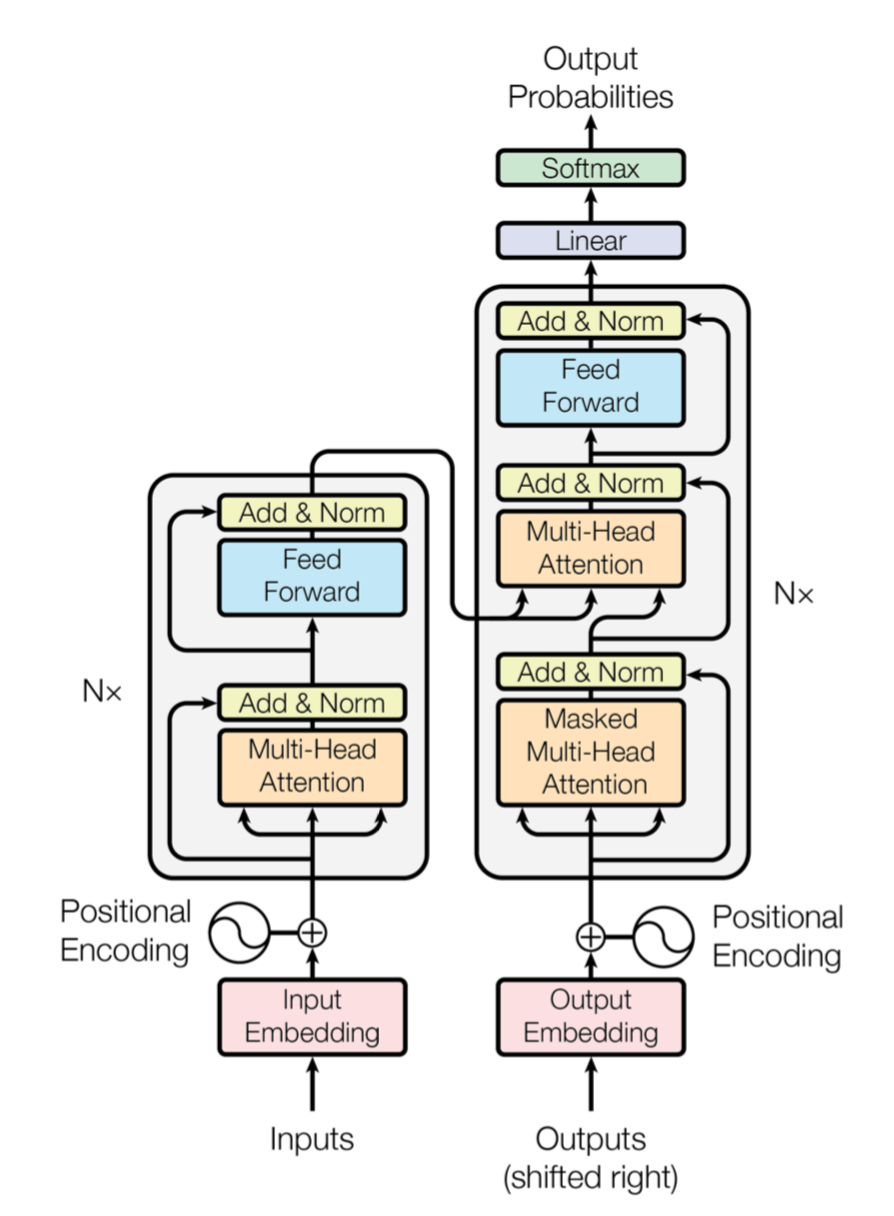
\includegraphics[width=.5\linewidth]{files/attention-1.png}
  \caption{Diagrammatical framework for transformer architecture \cite{attention}.}
  \label{fig:attention-1}
\end{figure}

The transformer \cite{attention} directly learns these dependencies rather than relying on the hidden state and the forget gates. In other words, the transformer removes the dependence on the distance between words when modeling dependencies between words. The transformer is an extension of the attention mechanism, which simply uses the hidden state from every cell to create a context vector that is combined with the encoder output as input to the decoder. The transformer attends over keys, values, and queries instead of word tokens. Typically, the keys and values are the encoder hidden states, while the query is the previous output of the decoder. Different linear transformations are applied to the output of the scaled dot-product attention with the formula in \ref{fig:attention-formula} to each "head" of attention. The number of heads is a tuning parameter, and having multi-head attention allows the model to weight the representation subspaces rather than simply averaging them. The multi-head attention is combined with feed-forward layers to construct an encoder-decoder model as shown in \ref{fig:attention-1}.

\begin{figure}
    \centering
    $$Att(Q,K,V) = softmax(\frac{QK^T}{\sqrt{d_k}})V$$
    \caption{Scaled dot-product attention, where $d_k$ is the dimensionality of the queries and keys.}
    \label{fig:attention-formula}
\end{figure}


\section{\label{sec:level4} Presentation of papers}
\subsection{Summary of Distributed Representations of Sentences and Documents}
% TODO: Summarize the motivation, goals, techniques and results of the paper. Fill {Paper 1} with the exact title of the paper as found in your .bib file. 
Doc2vec \cite{conf/icml/LeM14} learns embeddings for variable-length pieces of texts by predicting the next word in a sentence using shared word vectors to train a set of unique document vectors.  In this sense, "document", "paragraph" and "sentence" are equivalent, simply meaning some text of variable length. Paragraph vectors are unique to each paragraph, while word vectors are shared among different paragraphs. Similar to word2vec, doc2vec can be constructed with either of two learning objectives: distributed memory and distributed bag of words. The only difference between doc2vec and word2vec is that the weights depend on the words and documents in the former and just the words in the latter. Specifically, word2vec learns the objective in \ref{fig:word2vec-obj} while doc2vec learns the objective in \ref{fig:doc2vec-obj}.

\begin{figure}[h!]
    \centering
    $$y=b+Uh(w_{t-k}, ..., w_{t+k};W)$$
    \caption{Word2vec training objective, where U,b are softmax parameters, and h is the concatenation of word vectors from W}
    \label{fig:word2vec-obj}
\end{figure}

\begin{figure}[h!]
    \centering
    $$y=b+Uh(w_{t-k}, ..., w_{t+k};W,D)$$
    \caption{Doc2vec training objective, where U,b are softmax parameters, and h is the concatenation of word vectors from W and document vectors from D}
    \label{fig:doc2vec-obj}
\end{figure}

\begin{figure}[h!]
\centering
  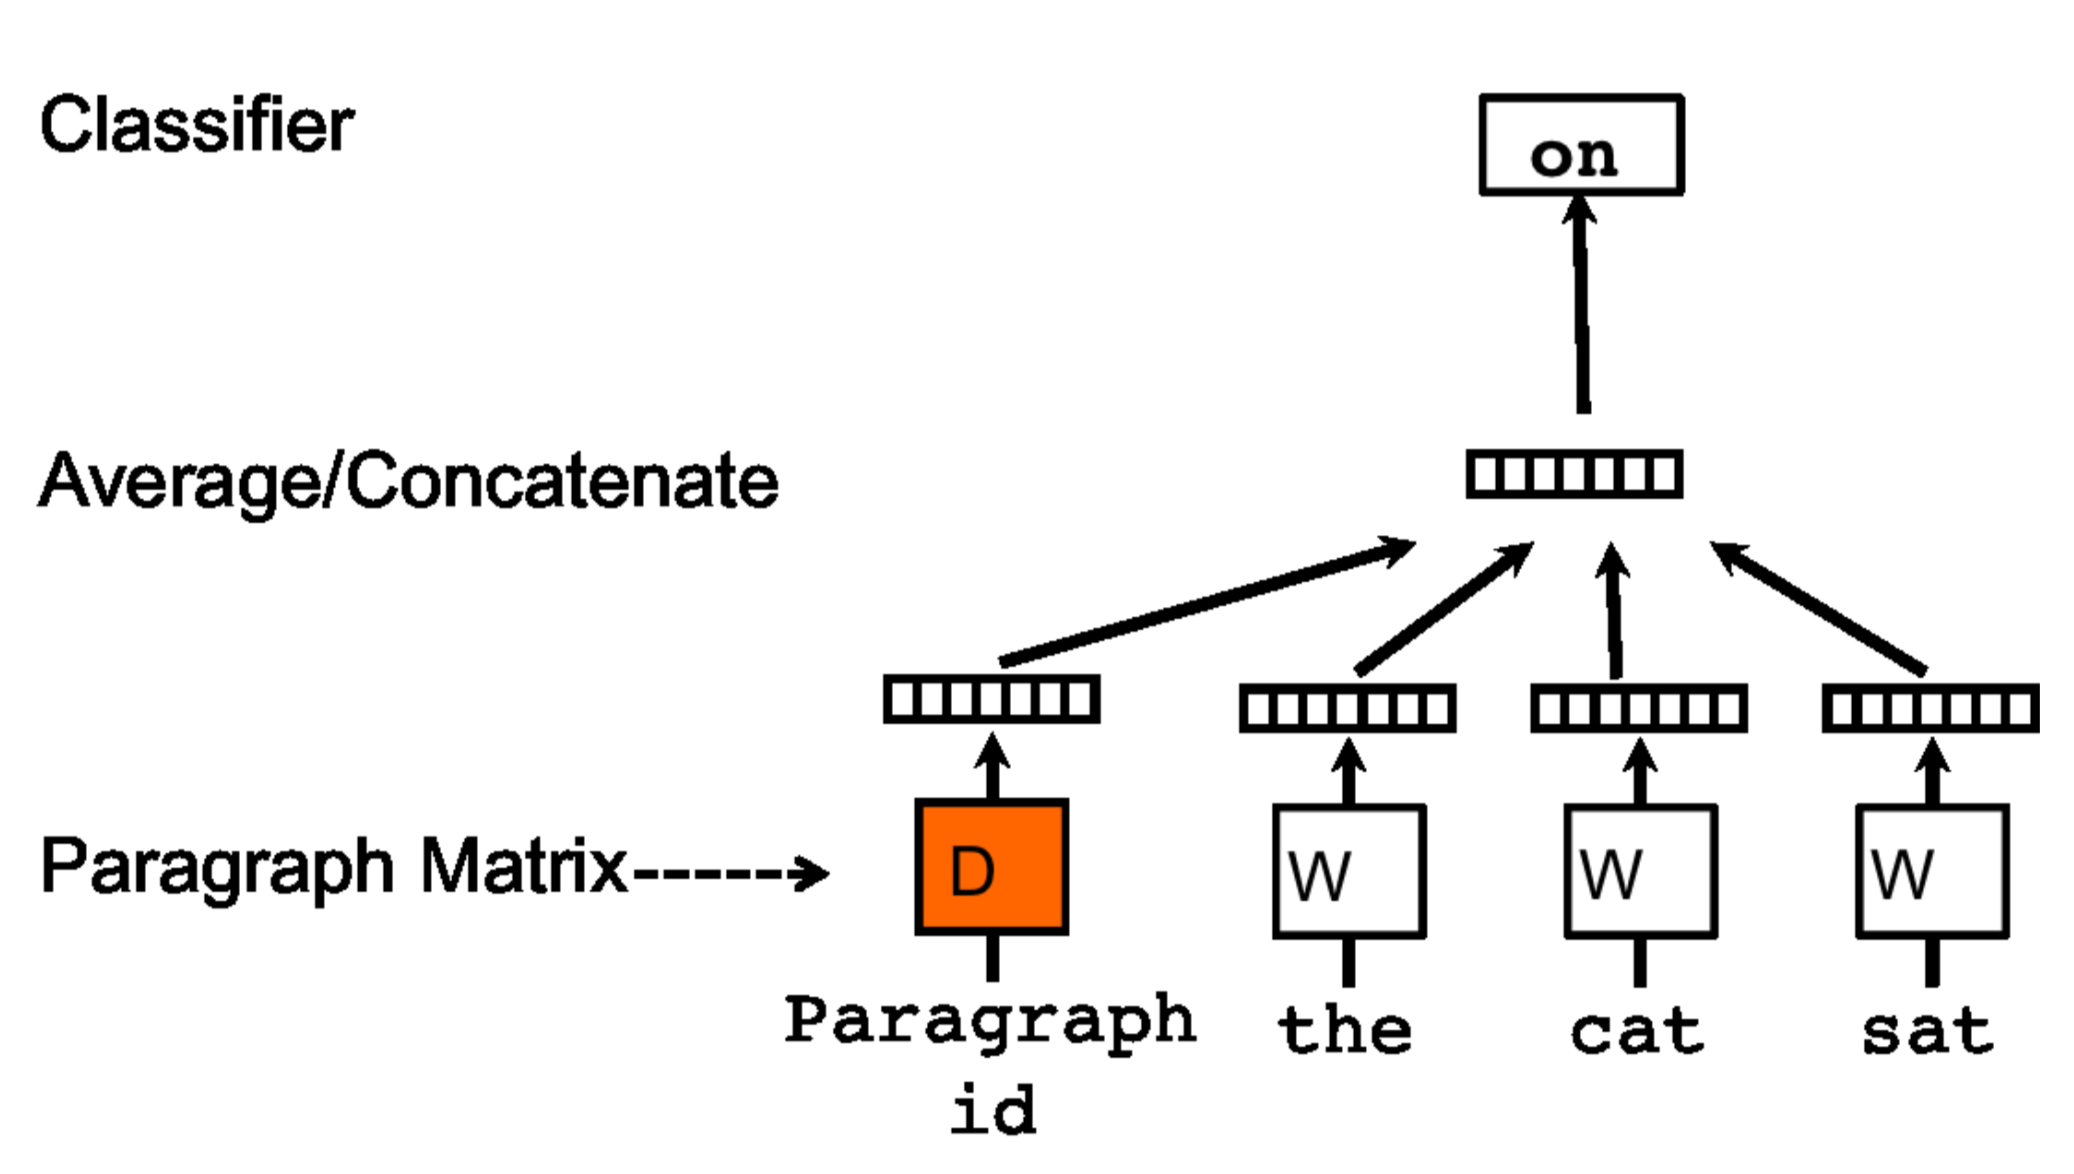
\includegraphics[width=.5\linewidth]{files/doc2vec-2.png}
  \caption{Diagrammatical framework for distributed memory approach to doc2vec.}
  \label{fig:doc2vec2}
\end{figure}

\begin{figure}[h!]
\centering
  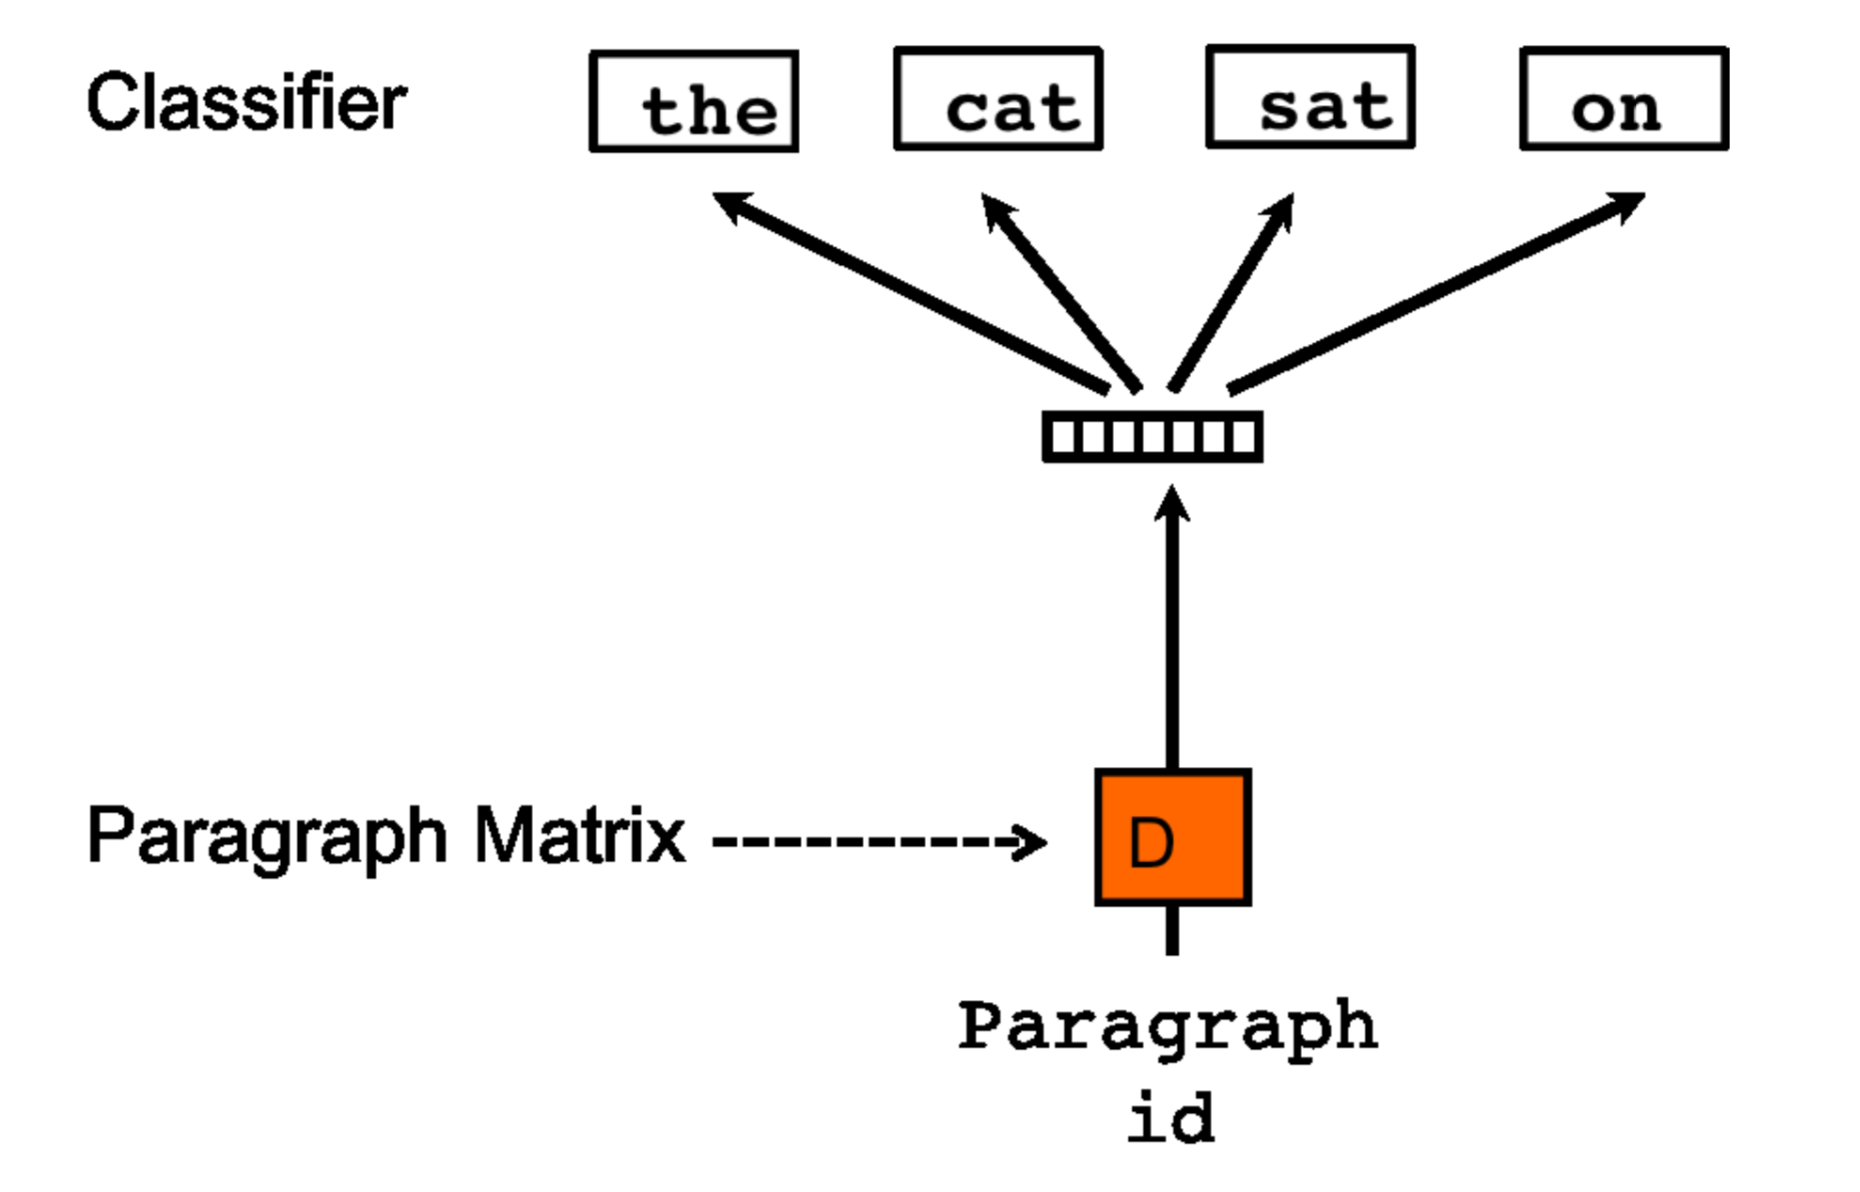
\includegraphics[width=.5\linewidth]{files/doc2vec-3.png}
  \caption{Diagrammatical framework for distributed bag of words approach to doc2vec.}
  \label{fig:doc2vec3}
\end{figure}

Figure \ref{fig:doc2vec2} shows the distributed memory approach to doc2vec. Randomly initialized word vectors and paragraph vectors are used to predict the next word in a sentence. At each training step, a fixed-length context is sampled from a random paragraph. The paragraph vector is shared across each context within paragraphs but not between paragraphs, and can be conceptualized as the topic of the paragraph. Over many training steps, many combinations of contexts from each paragraph converge to learn the embedding for the paragraph. Because paragraph vectors are learned for the training corpus, they must be inferred at prediction time. This is done by holding the rest of the parameters, word vectors, and softmax weights fixed, and adding more columns to the document matrix and gradient descending on it.

Figure \ref{fig:doc2vec3} shows the distributed bag of words approach to doc2vec. In this case, the objective is to predict randomly sampled words from the paragraph given the paragraph vector. This model is simpler, requires less storage, and is similar to the skip-gram approach in word2vec. While distributed memory tends to outperform distributed bag of words, the concatenation of both outperforms either individually. The authors thus recommend training both approaches and using concatenated paragraph embeddings for downstream tasks.

Doc2vec significantly improves upon word vectors in a number of downstream NLP tasks. Error rates are reduced by 2.4 and 3 percent for sentiment tagging using the stanford sentiment treebank dataset \ref{fig:doc2vec-res1}. Do2vec achieves a 7.42\% error rate on the IMBD sentiment classification task, a 16\% relative and 1.3\% overall improvement over the previous state of the art \ref{fig:doc2vec-res2}. Doc2vec also improves upon the previous state of the art for information retrieval. In an evaluation task with a goal of identifying pairs of similar sentences from triplet sets, doc2vec achieve an error rate of just 3.82\%, a 1.8\% absolute and 30\% relative improvement. These improvements are because doc2vec models word order in a lower dimensional space than previous large n-gram models did.

%\begin{figure}
%\centering
%  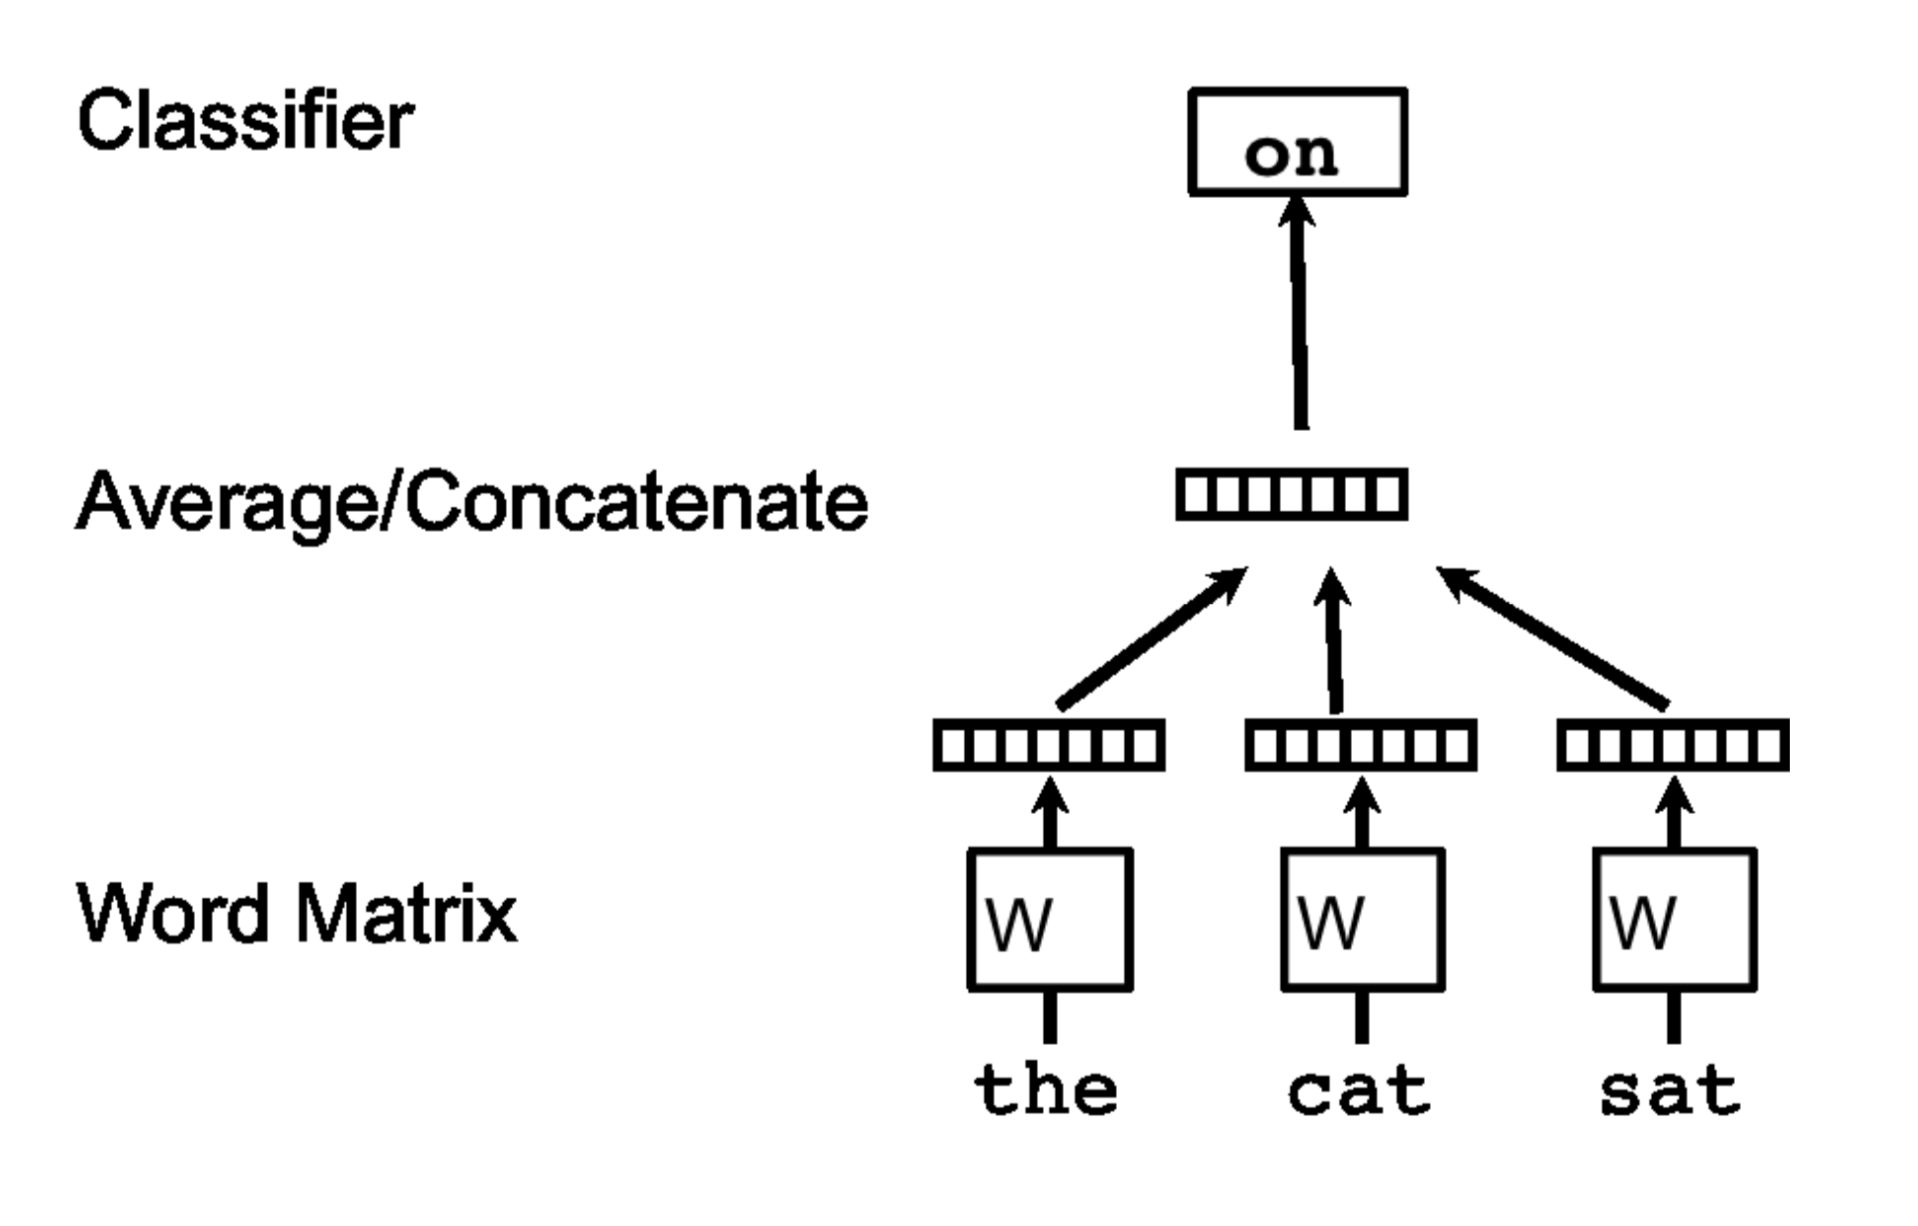
\includegraphics[width=.5\linewidth]{files/doc2vec-1.png}
%  \caption{Diagrammatical framework for word2vec.}
%  \label{fig:vae}
%\end{figure}

\begin{figure}
\centering
  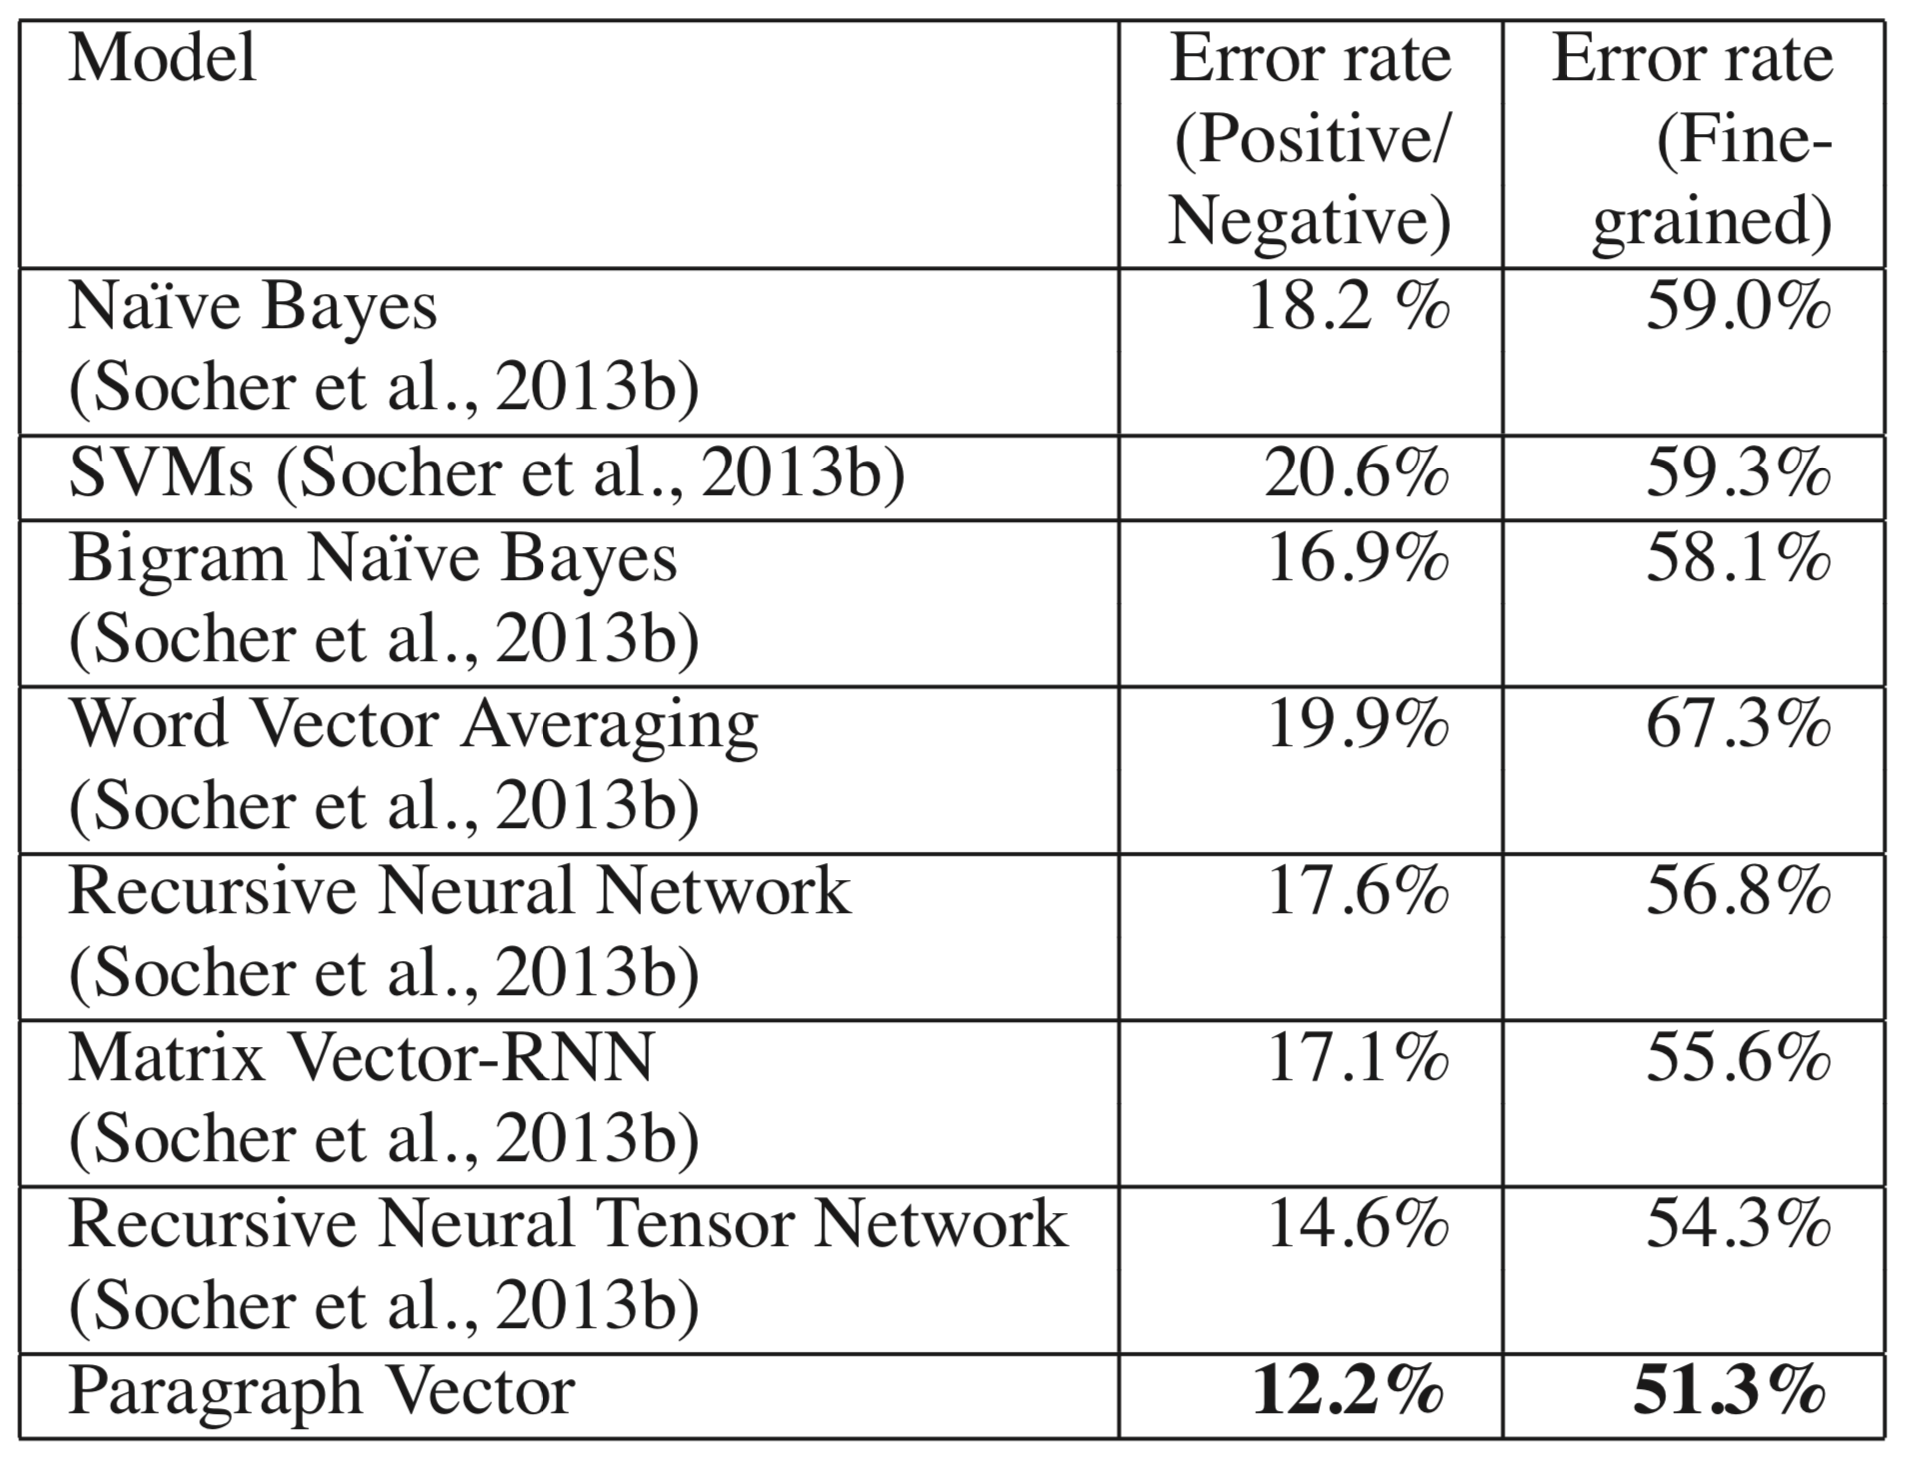
\includegraphics[width=.7\linewidth]{files/doc2vec-4.png}
  \caption{Results of doc2vec on sentiment analysis for the Stanford treebank task.}
  \label{fig:doc2vec-res1}
\end{figure}

\begin{figure}
\centering
  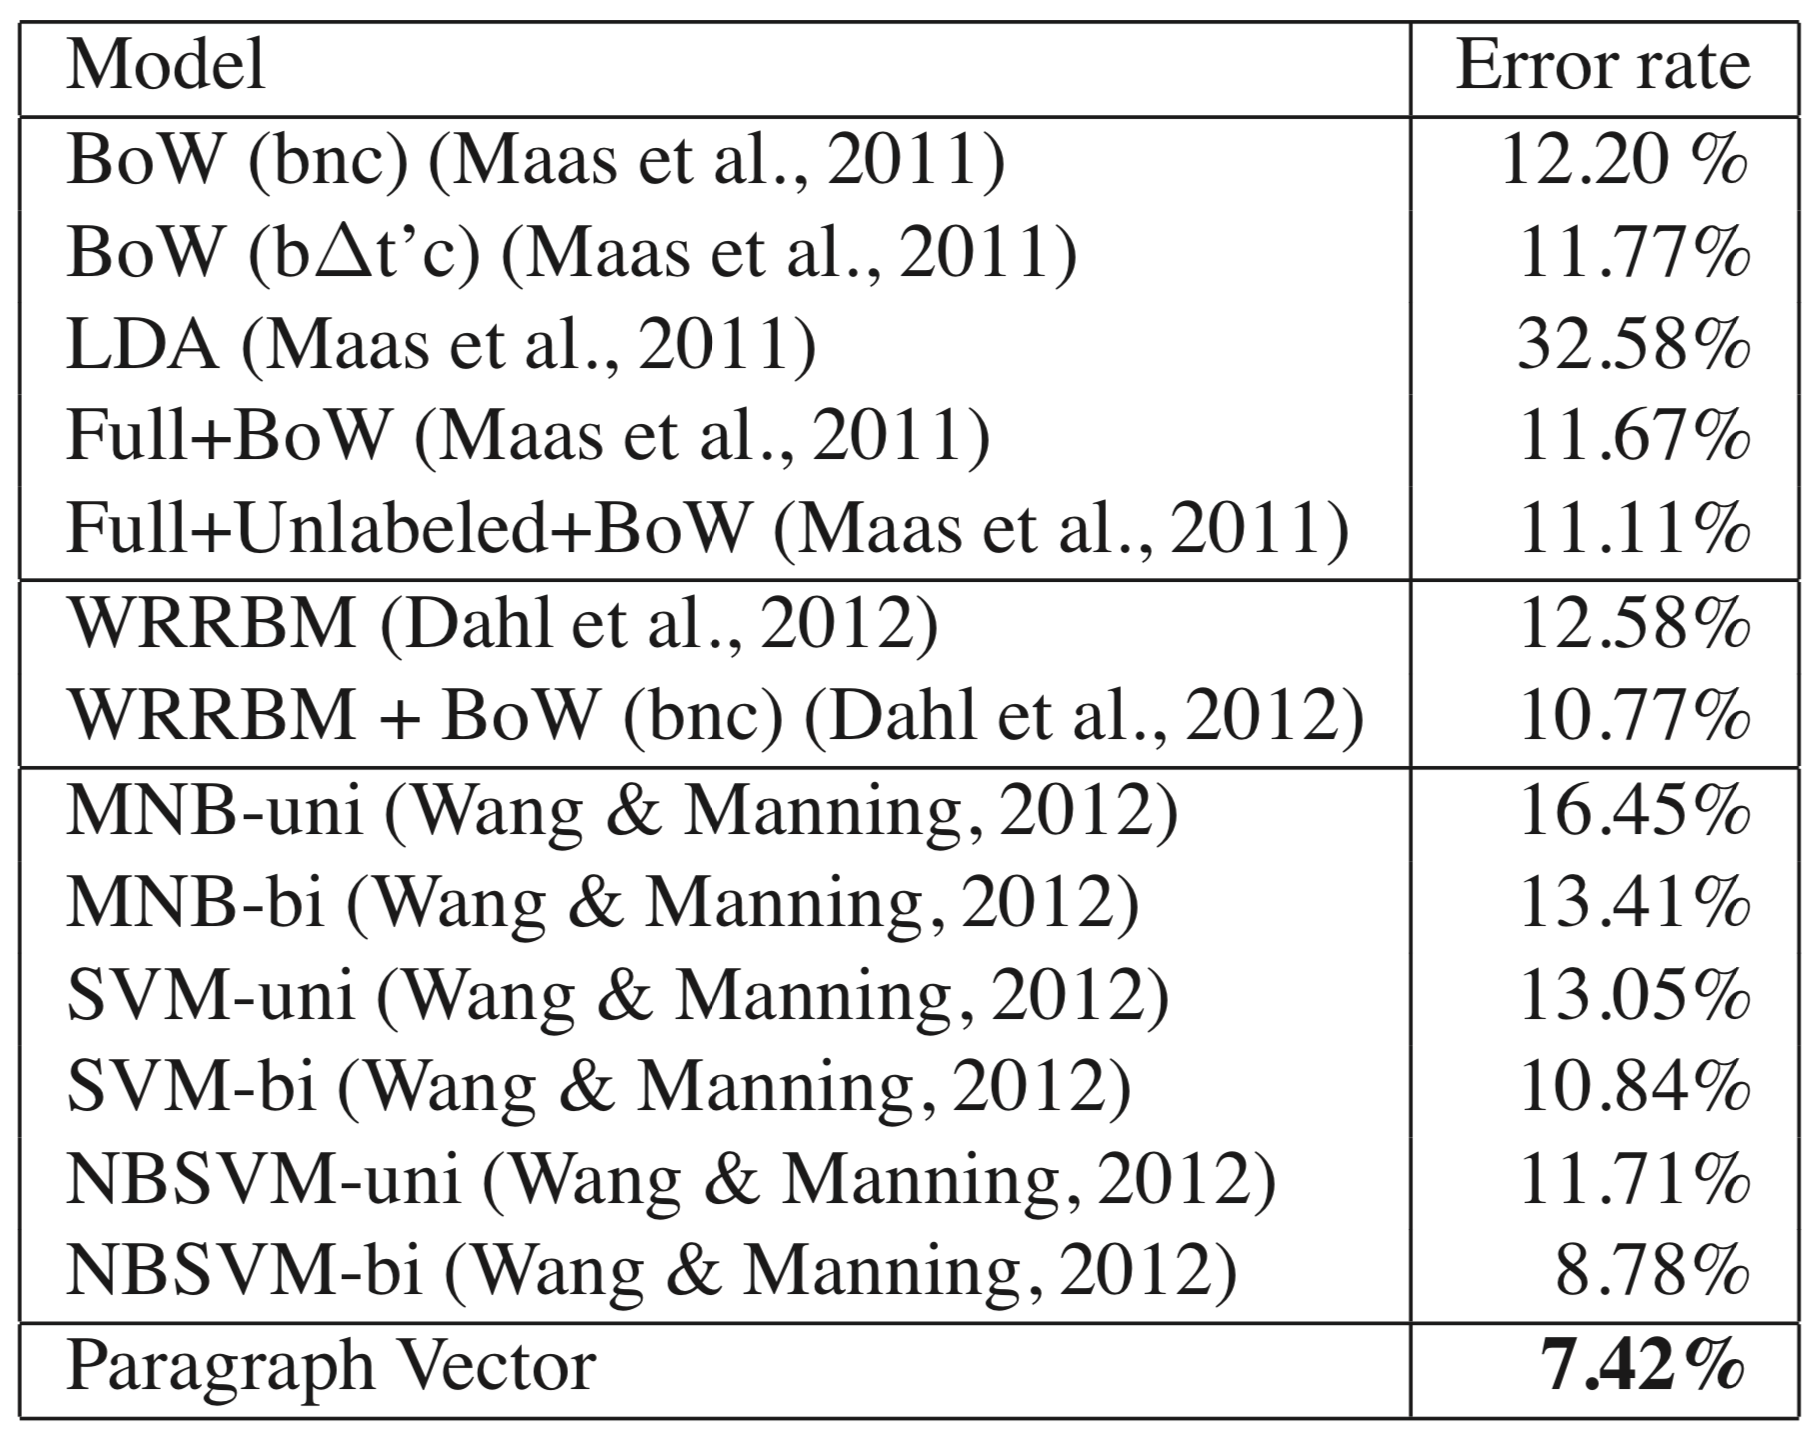
\includegraphics[width=.7\linewidth]{files/doc2vec-5.png}
  \caption{Results of doc2vec on sentiment analysis for the IMDB task.}
  \label{fig:doc2vec-res2}
\end{figure}

%\begin{figure}
%\centering
%  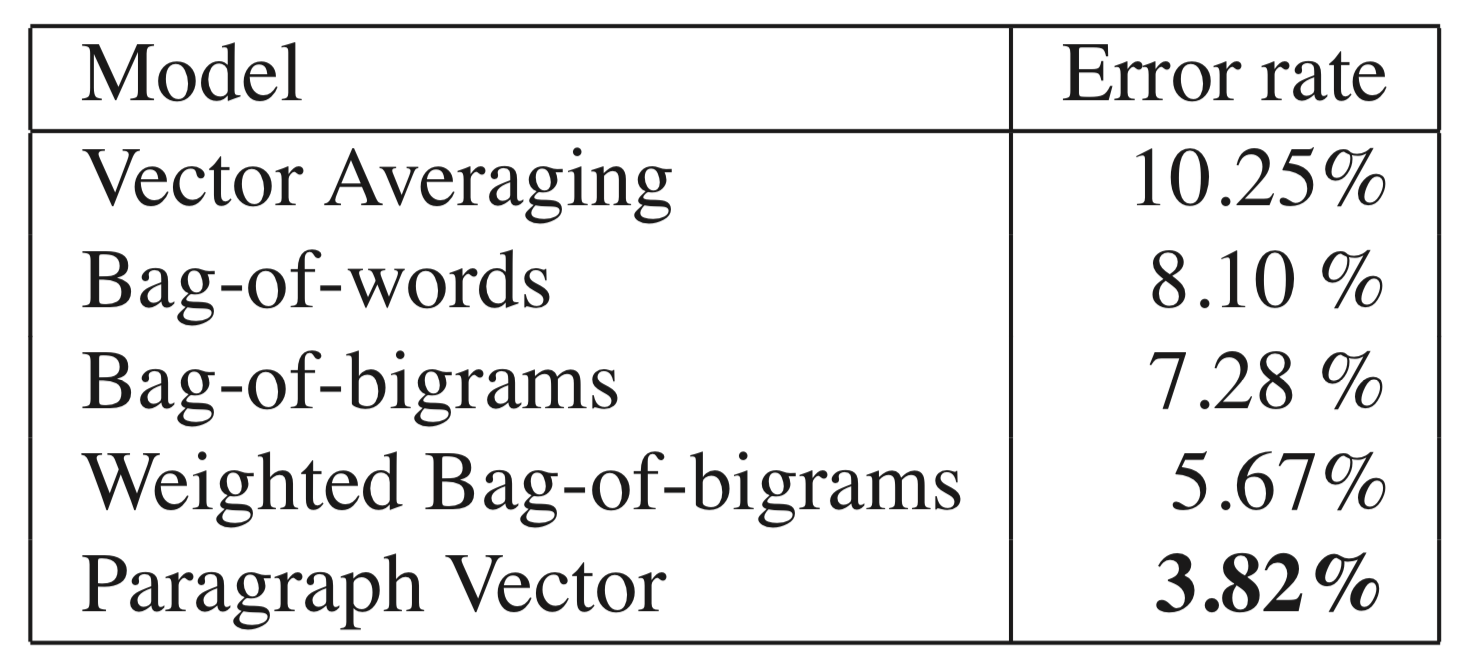
\includegraphics[width=.5\linewidth]{files/doc2vec-6.png}
%  \caption{Results of doc2vec on neural information retrieval.}
%  \label{fig:doc2vec-res3}
%\end{figure}


\subsection{Summary of Skip-thought Vectors}
% TODO same as previous subsection

Skip thoughts (\cite{DBLP:journals/corr/KirosZSZTUF15}) addresses issues of generalizability in doc2vec and previous recursive and recurrent methods. Skip thoughts abstracts the skip-gram approach of word2vec to the sentence level. Trained on 11,000 books in the public domain, skip thoughts is an off-the-shelf unsupervised sentence encoder. The encoder-decoder model is formulated with a goal of reconstructing surrounding sentences given an input sentence, such that similar sentences are mapped to similar vector representations (Figure \ref{fig:skipthoughts-1}). 

\begin{figure}[h!]
\centering
  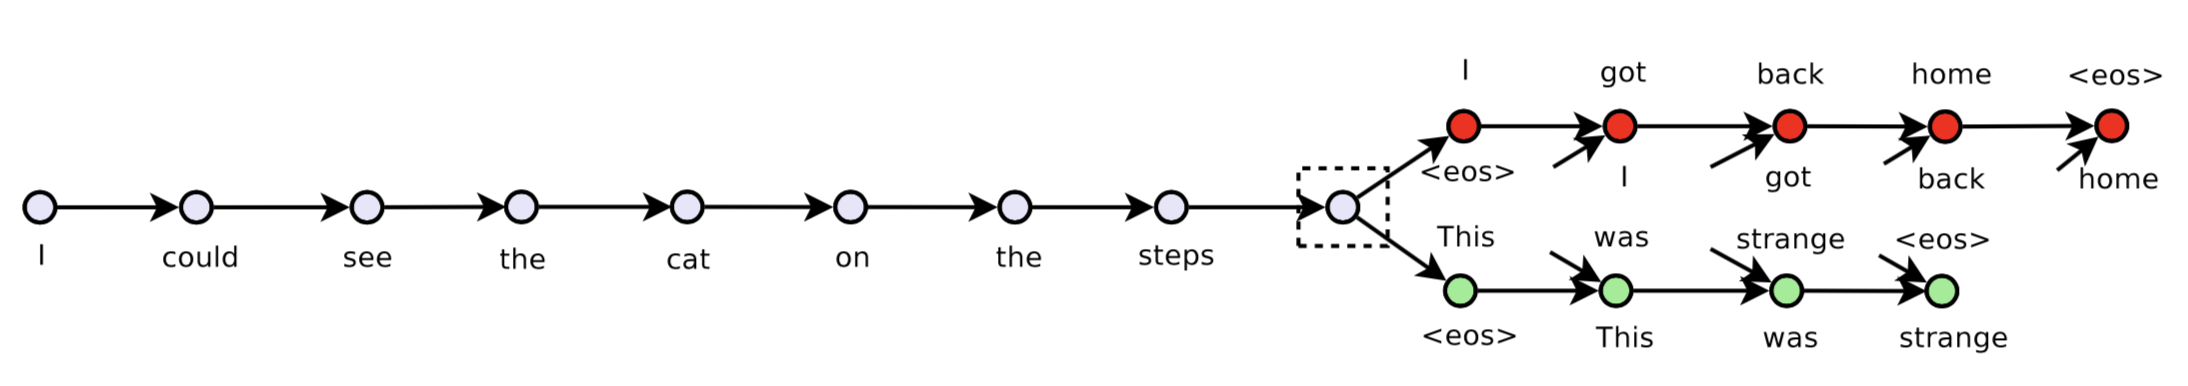
\includegraphics[width=.8\linewidth]{files/skipthoughts-1.png}
  \caption{Model architecture for skip-thoughts vectors. Colors represent sharing of parameters. Unconnected arrows are attached to the output of the encoder.}
  \label{fig:skipthoughts-1}
\end{figure}

The encoder maps words to sentences using an RNN with GRU activation, while the decoder generates surrounding sentences. If $w_i^1...w_i^n$ are words in a sentence, and $x_i...x_n$ are the word2vec embeddings for each word, the encoder produces a hidden state $h_i^t$ which is the sentence representation up to word t. Thus, $h_i^n$ is the representation for the full sentence, where n is equal to the length of the sentence. The encoder formula is elaborated in Figure \ref{fig:skipthoughts-encoder}, where $\bar h$ is the proposed state update, $z$ is the update gate, and $r$ is the reset gate. 

\begin{figure}[h!]
    \centering
    \begin{align*}
    r^t &= \sigma(W_rx^t + U_r h^{t-1}) \\
    z^t &= \sigma (W_z x^t + U_z h^{t-1}) \\
    \bar h^t &= tanh(Wx^t + U(r^t \cdot h^{t-1})) \\
    h^t &= (1 - z^t) \cdot h^{t-1} + z^t \cdot \bar h ^t
    \end{align*}
    \caption{Encoder model for skip-thoughts, where $\bar h$ is the proposed update, z is the update gate, and r is the reset gate.}
    \label{fig:skipthoughts-encoder}
\end{figure}

The decoder (\ref{fig:skipthoughts-decoder} is similar to the encoder except it introduces matrices $C_z$, $C_r$, and $C$. These bias the update, reset, and hidden states by the sentence vector. There are separate decoders for the previous and the next sentence, which share parameters except for the vocabulary matrix. The objective, shown in \ref{fig:skipthoughts-obj} is to, given a tuple, maximize the sum of the log probabilities of the first and last sentences conditioned on the encoded middle sentence. 

\begin{figure}[h!]
    \centering
    \begin{align*}
    r^t &= \sigma(W_r^d x^{t-1} + U_r^d h^{t-1} _  C_r h_i) \\
    z^t &= \sigma (W_z^d x^{t-1} + U_z h^{t-1} + C_z h_i) \\
    \bar h^t &= tanh(W^d x^{t-1} + U^d(r^t \cdot h^{t-1}) + C h_i) \\
    h^t_{i+1} &= (1 - z^t) \cdot h^{t-1} + z^t \cdot \bar h ^t \\
    P(w^t_{i+1}|w^{<t}_{i+1}, h_i) &\propto exp(v_{w^t_{i+1}}v_{h^t_{i+1}})
    \end{align*}
    \caption{Decoder model for skip-thoughts, where $\bar h$ is the proposed update, z is the update gate, r is the reset gate, $V_{w^t_{i+1}}$ denotes the row of V corresponding to the word of $W^t_{i+1}$.}
    \label{fig:skipthoughts-decoder}
\end{figure}

\begin{figure}
    \centering
    $$
    \sum\limits_{t}logP(w^t_{i+1}, h_i) + \sum\limits_{t}log P (w^t_{i-1}|w^{<t}{i-1}, h_i)
    $$
    \caption{Objective for skip thoughts model.}
    \label{fig:skipthoughts-obj}
\end{figure}

Skip-thoughts also introduces a mechanism to expand vocabulary to incorporate out of vocabulary words. It does so by using an un-regularized L2 linear regression for the matrix W that maps the word2vec vocabulary to the RNN vocabulary. W is equal the encoder vocabulary space divided by the word2vec embedding space. This allows any word with a word2vec embedding to be mapped into the encoder's vocabulary space.

Skip-thoughts is tested on eight different tasks, including semantic relatedness, paraphrase detection, image-sentence ranking, classification, and four different sentiment and subjectivity tests. A linear classifier, with no fine-tuning or back-propagation or additional feature engineering, is used in all evaluation cases in order to test the generalizability and ease-of-use of skip-thoughts. The authors test a uni-directional model, as well as a bi-directional model concatenating the embeddings of correctly ordered and reversed sentences. The uni- and bi- models are also concatenated to form a combine-skip model.

For the semantic relatedness task, the goal is to, given two sentences, generate a score of how related the sentences are based on human evaluation. Previous approaches used heavily feature engineered data learned specifically for the task. Skip-thoughts uses no feature engineering and is a general embedding, but performs on-par to the more complicated models. Figure \ref{fig:skip-thoughts-sr} shows example sentence pairs and compares the predicted and ground truth relatedness. Skip-thoughts performs well on many challenging cases, identifying differences due to negation, changing direct and indirect objects, and active and passive verbs. However, skip-thoughts fails to identify small distinctions that affect meaning, such as polysemes and more complicated verb changes.

\begin{figure}
\centering
  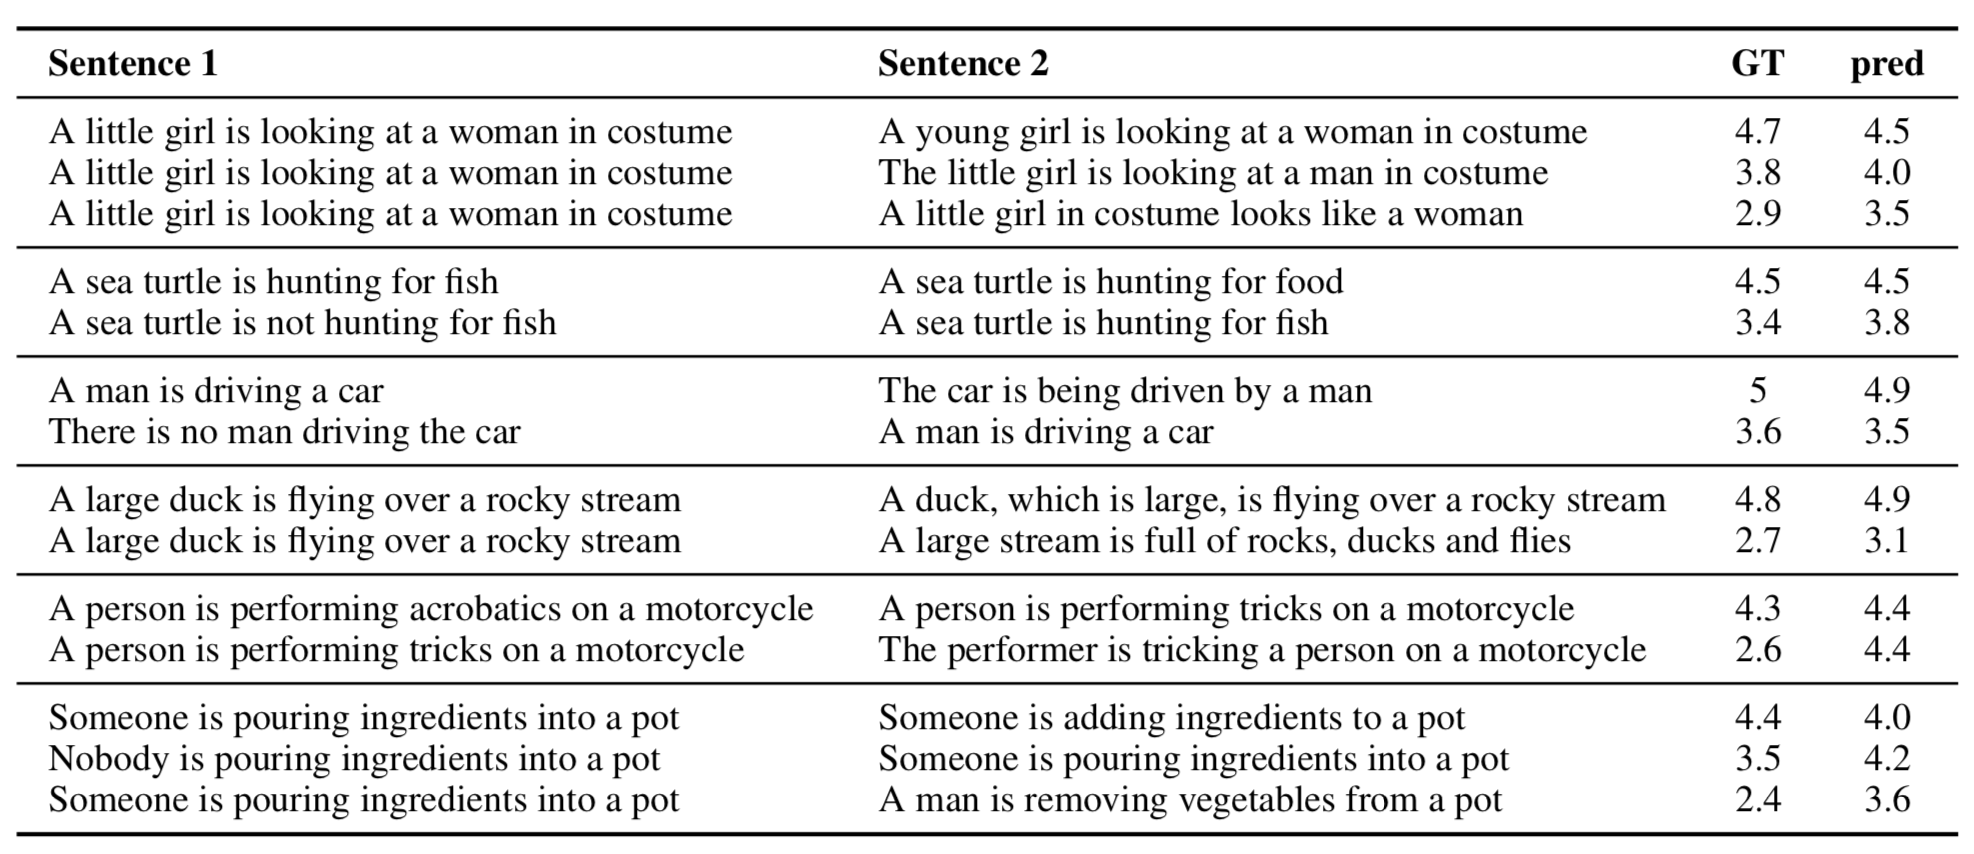
\includegraphics[width=1\linewidth]{files/skipthoughts-5.png}
  \caption{Example predictions from the SICK evaluation task. GT is the human-scored relatedness from 1 to 5.}
  \label{fig:skip-thoughts-sr}
\end{figure}

Similarly to the semantic relatedness task, previous paraphrase detection models made extensive use of feature engineering. The goal of paraphrase detection is to, given two sentences, predict whether one is the paraphrase of the other. Using logistic regression alone, all three models (uni, bi, and combine) fail to outperform any of the baselines, with F1 scores of 81.9, 81.2, and 82.0, respectively. However,  the combine-skip model combined with sentence statistics achieves an F1 score of 83.0, much closer to the state of the art of 84.1.

Image-sentence ranking is evaluated using the Microsoft COCO dataset where each image has five human-generated captions. Skip-thoughts is evaluated on image annotation, where candidate annotations are ranked by relevance, and image search, where images are ranked given an annotation. The combine-skip thoughts model performs 5-10\% relatively worse than RNN-based models that learn jointly learn the embeddings specifically for the annotation and search tasks. 

Skip-thoughts is evaluated on five different classification datasets: movie review sentiment (MR), customer product reviews (CR), subjectivity/objectivity classification (SUBJ), opinion polarity (MPQA), and question-type classification (TREC). All classification is done with a logistic regression regularized with an L2 penalty. The results are shown in figure X, demonstrating that skip-thoughts performs similarly to bag-of-words baselines but worse than models trained directly for classification.

%\begin{figure}
%\centering
%  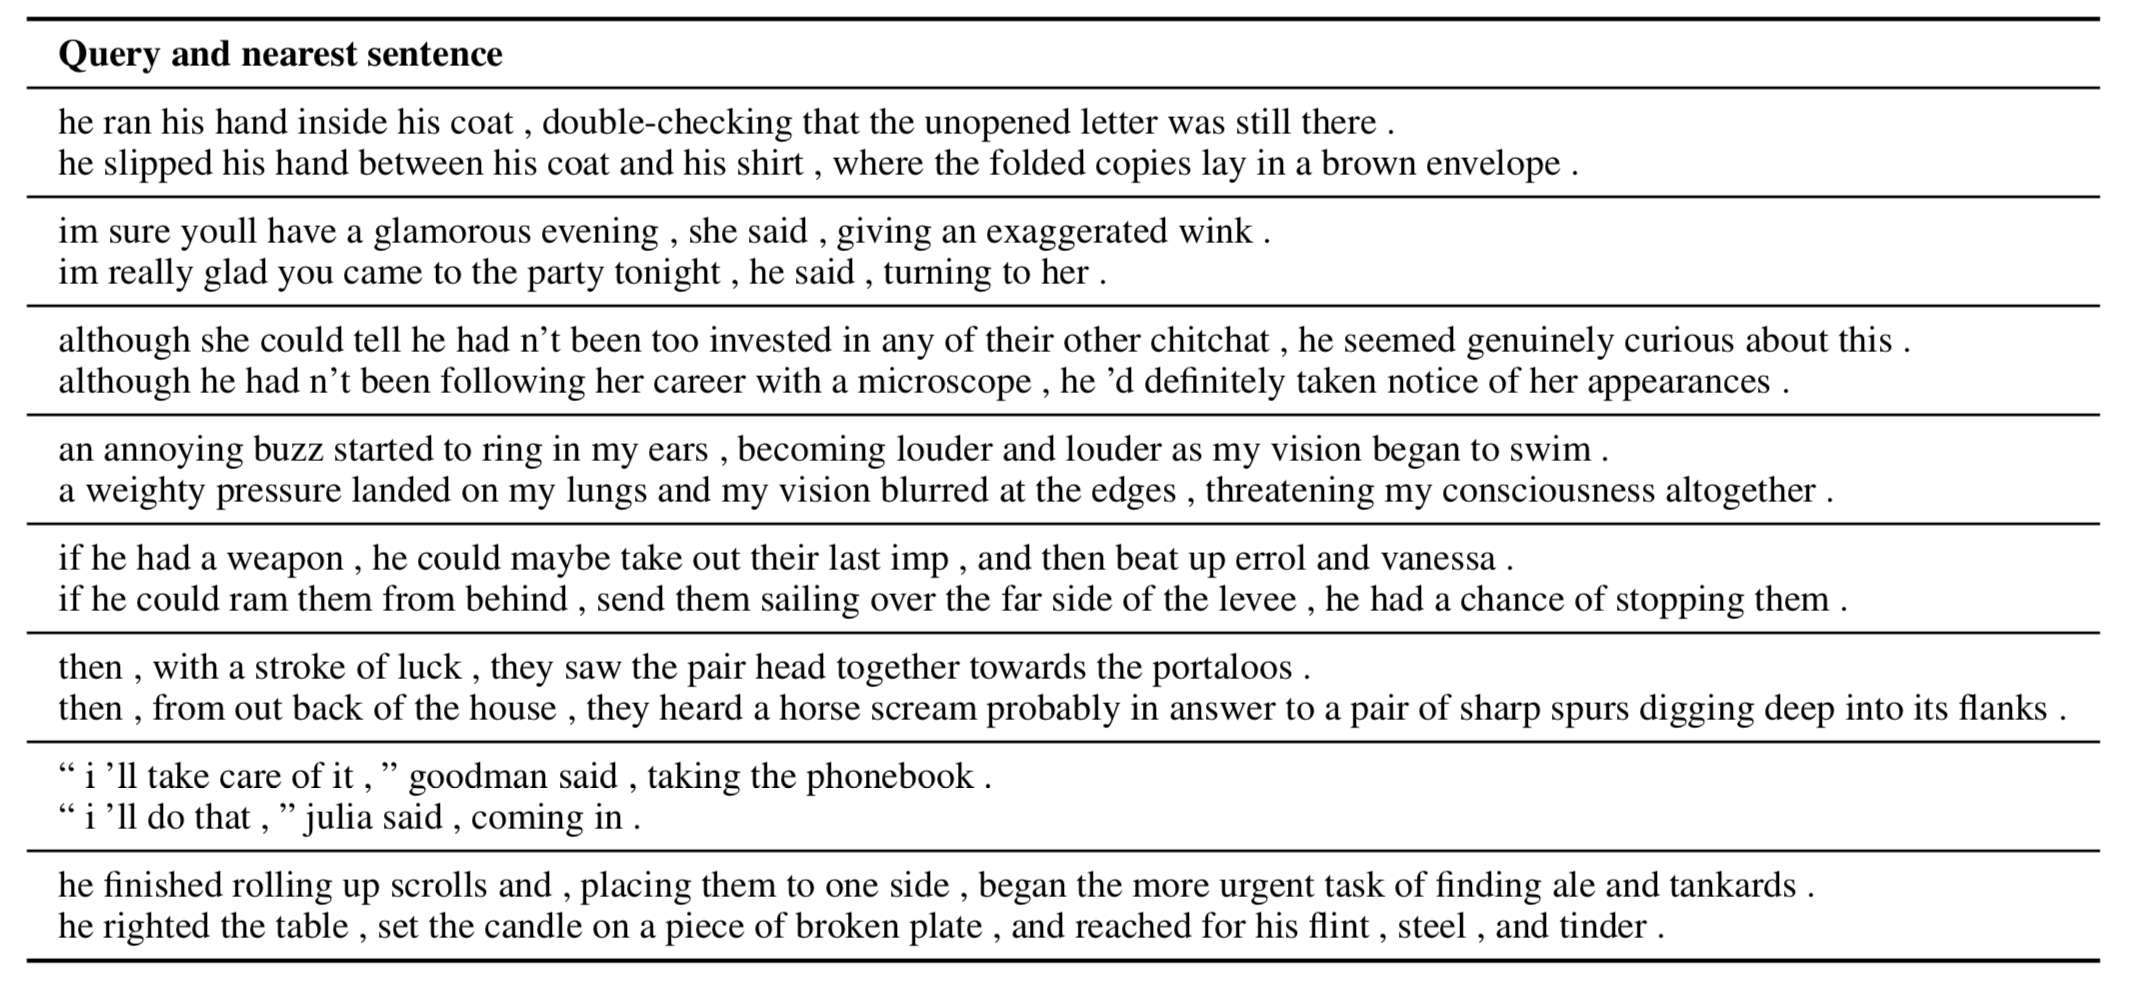
\includegraphics[width=.8\linewidth]{files/skipthoughts-2.png}
% \caption{Do I keep 1.}
%  \label{fig:vae}
%\end{figure}

\begin{figure}[h!]
\centering
  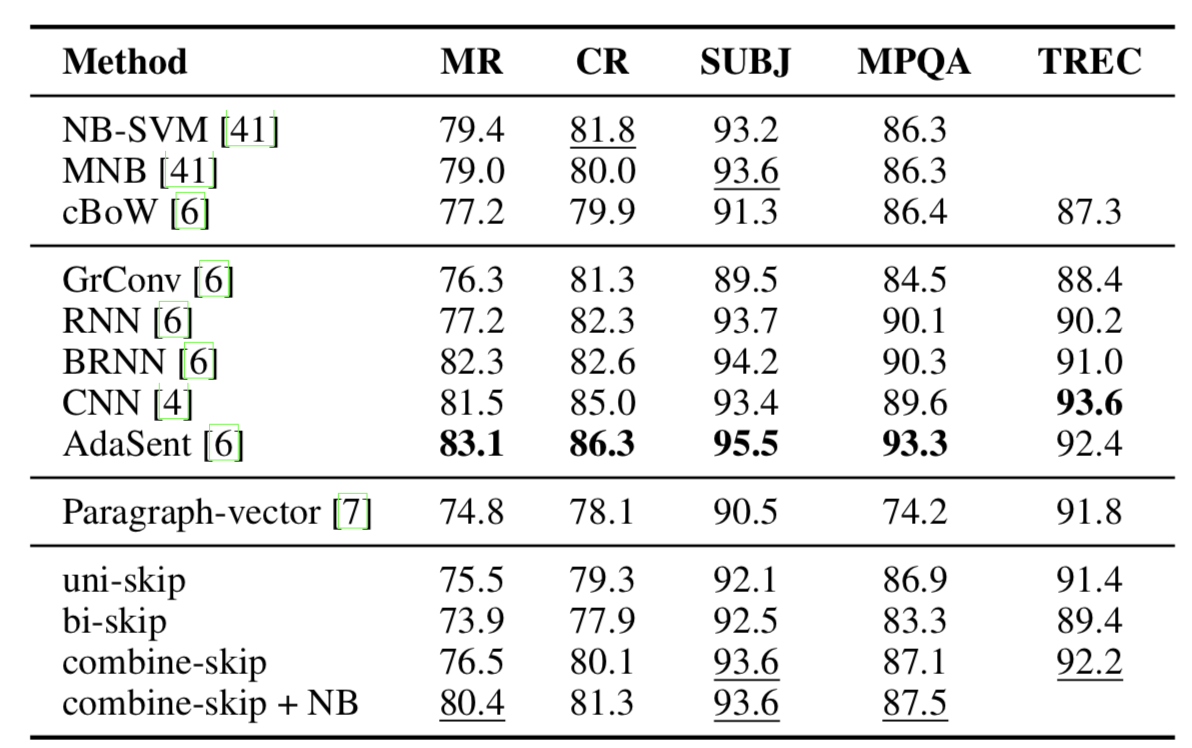
\includegraphics[width=.7\linewidth]{files/skipthoughts-8.png}
  \caption{Classification accuracy on five classification tasks, grouped into, from top to bottom, bag-of-words, supervised, paragraph vector, and skip-thoughts.}
  \label{fig:vae}
\end{figure}

\subsection{Summary of An Efficient Framework for Learning Sentence Representations}
% TODO same as previous subsection

Quick thoughts  \cite{logeswaran2018an} are unsupervised sentence representations that address a number of issues with previous sentence embeddings: the inability to model multiple ways of expressing ideas, sensitivity to sentence structure, and high computational costs. Rather than using a generative approach, quick thoughts uses a discriminative approximation to attempt to identify the embedding of a context sentence given a set of candidate sentences (Figure \ref{fig:quickthoughts-1}). The conceptual basis for this approach is that the topic or meaning of a sentence is encoded in the information that allows an embedding to predict the information about contextual sentences. 


\begin{figure}[h!]
\centering
  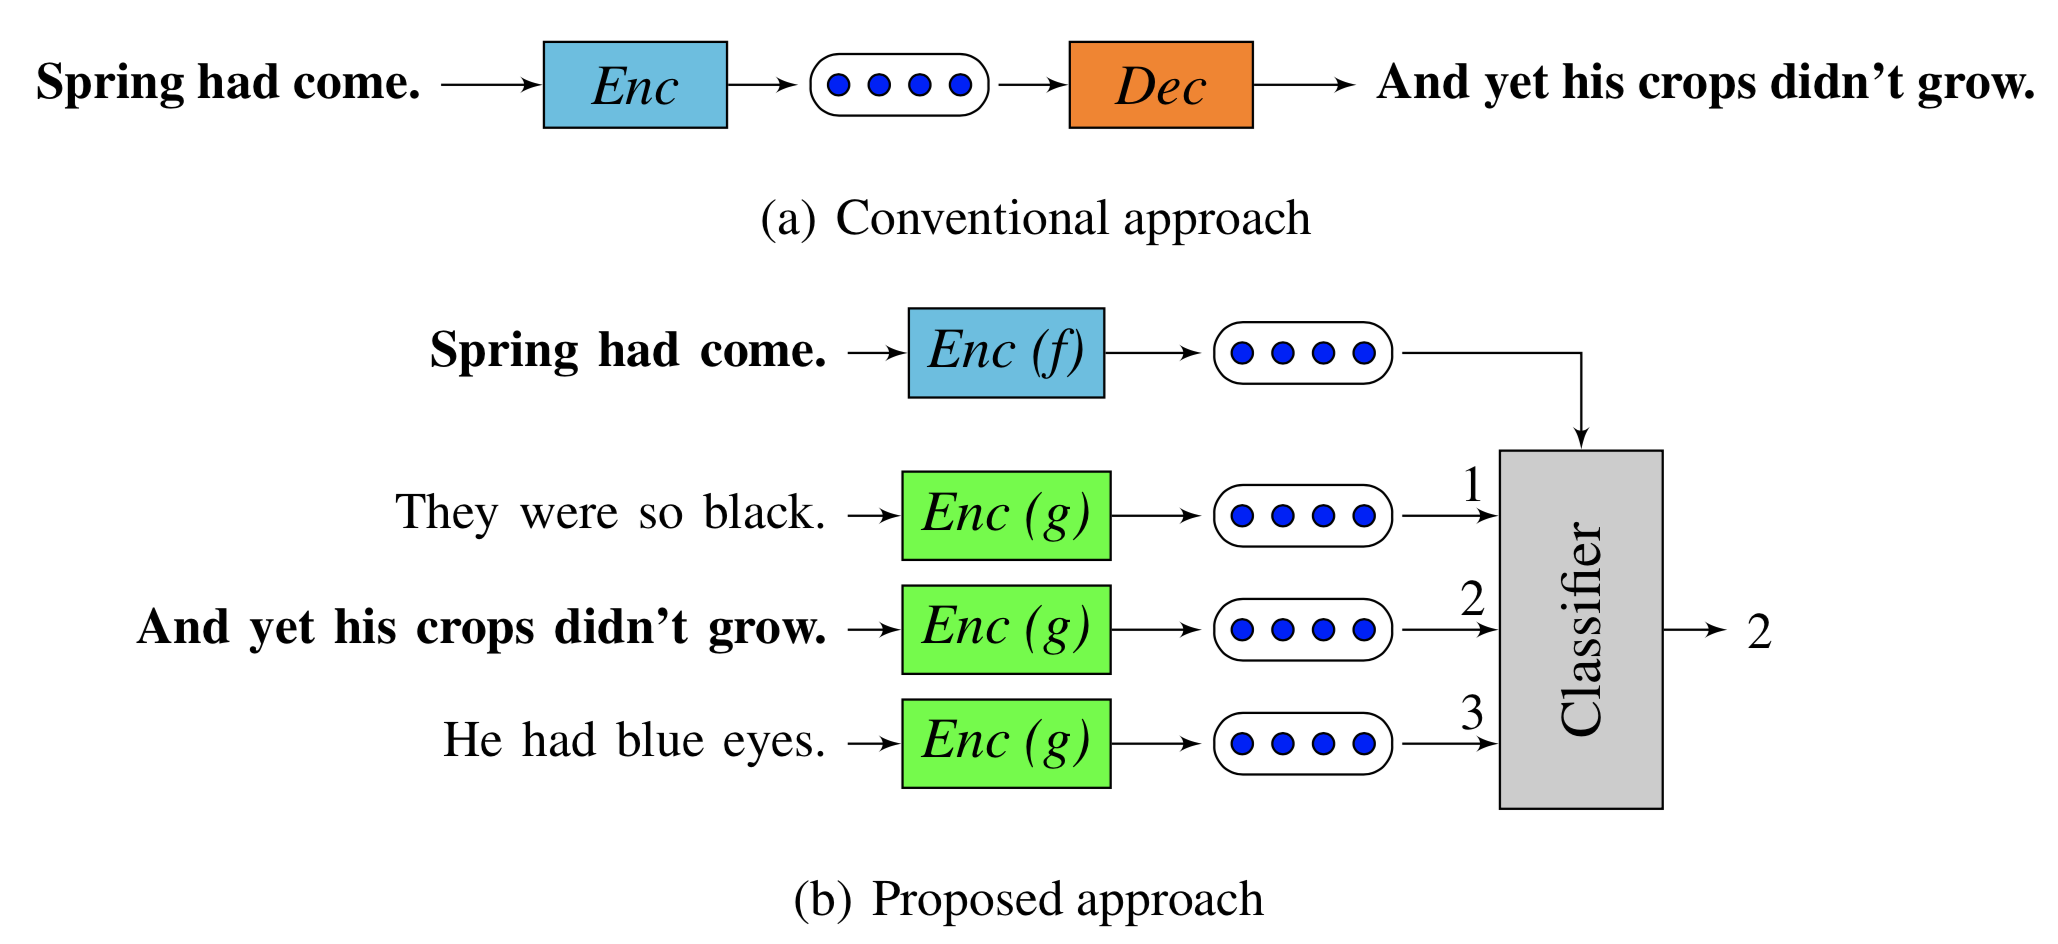
\includegraphics[width=.8\linewidth]{files/quickthoughts-1.png}
  \caption{Cap.}
  \label{fig:quickthoughts-1}
\end{figure}

Given an input sentence, quick-thoughts calculates the probability that each candidate sentence is a context sentence within the input with the equation in Figure \ref{fig:quickthoughts-obj}. The authors construct minibatches of 400 contiguous sentences, where all the sentences constitute the candidate pool S\textsubscript{cand}, which contains one context and many non-context sentences. In \ref{fig:quickthoughts-prob}, $c$ is a scoring function that is empirically chosen as the inner product of $u$ and $v$ in order to force the encoder to not rely upon a heavily engineered scoring function. The functions $f$ and $g$ are recurrent neural networks with GRU activation and no shared parameters. The outputs of $f$ and $g$ are concatenated at test time. The objective of quick-thoughts is to maximize the sum of the log probability of correctly identifying the context sentence for all minibatches of all input sentences (Equation \ref{fig:quickthoughts-obj}).


\begin{figure}[h!]
    \centering
    $$
    p(S_{cand}|s, S_{cand}) = \frac{exp[c(f(s),g(s_{cand}))]}{\sum exp[c(f(s),g(s'))]}
    $$
    \caption{Probability function for quick-thoughts}
    \label{fig:quickthoughts-prob}
\end{figure}

\begin{figure}[h!]
    \centering
    $$
    \sum\limits_{s \in D} \sum\limits_{s_{ctxt} \in S_{ctxt}} log p(s_{ctxt} | s, S_{cand})
    $$
    \caption{Objective for quick-thoughts.}
    \label{fig:quickthoughts-obj}
\end{figure}

Quick-thoughts is trained on 7,000 novels in the BookCorpus dataset, containing 45 million sentences, as well as the UMBC corpus with 129 million sentences derived from 100 million web pages. The model was trained to predict the previous and next sentence by encoding the middle sentence, though it would be possible to choose a wider context window. The RNNs are single-layered with randomly initialized GRU weights and word embeddings randomly initialized from -0.1 to 0.1. The authors test multiple versions of quick-thoughts. Uni-QT uses uni-directional RNNs for $f$ and $g$, bi-QT concatenates the forward and backward RNNs for $f$ and $g$, and combine-QT concatenates the embeddings from uni-QT and bi-QT. Quick-thoughts is also trained using pre-trained word vectors, randomly initialized and learned word vectors, and a combination of pre-trained and learned word vectors referred to as MC-QT. 

Quick-thoughts is evaluated on a number of classification tasks against bag-of-words, skip-thoughts, paragraph vectors, supervised methods, and task-specific supervised methods. Table \ref{fig:quickthoughts-res1} compares the performance of quick-thoughts with other unsupervised approaches. Combine-QT outperforms uni-QT and bi-QT on all tasks. Combining pre-trained and learned word vectors improves upon both the pre-trained and the learned word vectors models. Multichannel quick-thoughts improves upon the best skip-thoughts model on all tasks with just 8\% the training time (28 versus 336 hours). Quick-thoughts also performs competitively against supervised methods (Table \ref{fig:quickthoughts-res2}), improving upon the best baseline (InferSent) in six of eight cases despite not being supervised. An ensemble of weighted average predictions of models with variations in model type, embeddings, and training data performed competitively against task-specific supervised approaches (Figure \ref{fig:quickthoughts-res3}). Quick-thoughts performs better than previous pre-trained unsupervised methods on image annotation and image search, improving upon skip-thoughts by between between 2 and 4\% absolute accuracy, but fails to improve upon directly supervised models, performing between 8 and 22\% worse than the best baseline.

The main contribution of this paper is that the quick-thoughts algorithm attains similar accuracy as task-specific models tuned end-to-end on many tasks. Quick-thoughts trains nearly five times as fast as skip-thoughts (6.5 hours and 31 hours, respectively) and has only 20 million parameters, versus the 58 million of skip-thoughts. Additionally, quick-thoughts can train high-quality low-dimensional models, as reducing the em bedding size from 5,600 to 1,600 only drops performance averaged over all classification benchmarks from 86.7\% to 84.6\%. 

\newpage

\begin{figure}[h!]
\centering
  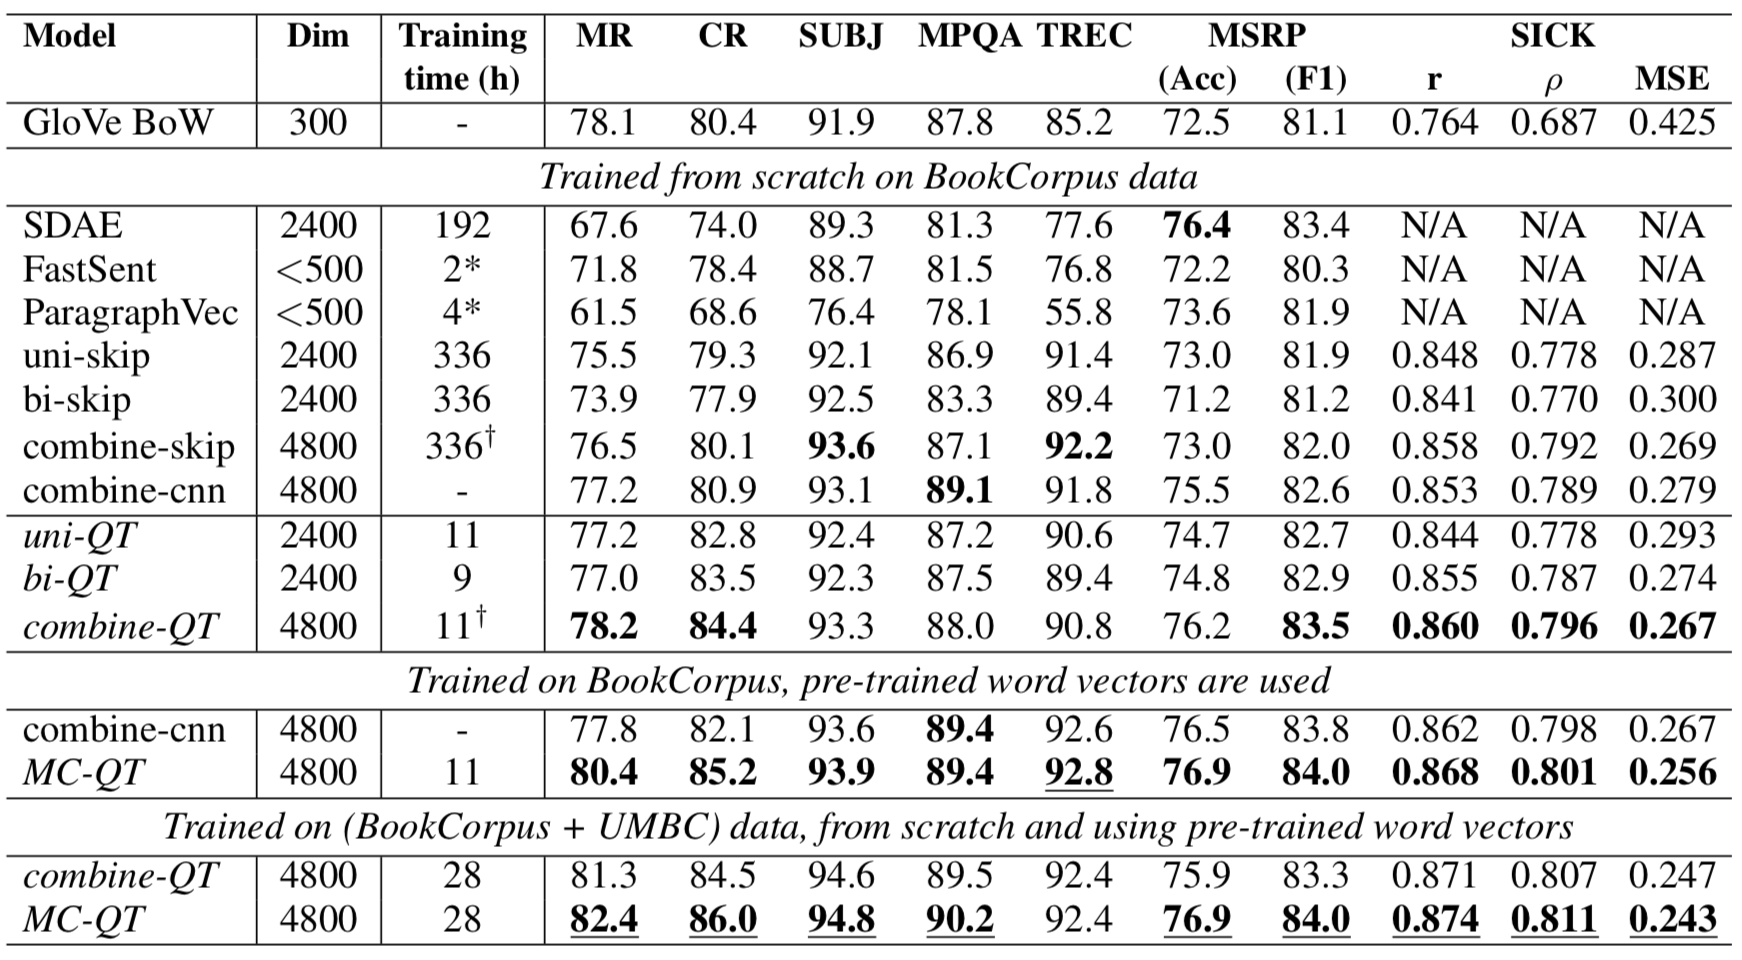
\includegraphics[width=1\linewidth]{files/quickthoughts-2.png}
  \caption{Comparison of quick-thoughts with other unsupervised approaches on the movie reviews (MR), product reviews (CR), subjectivity (SUBJ, opinion polarity (MPQA), question type classification (TREC), paraphrase identification (MSRP), and semantic relatedness (SICK) tasks.}
  \label{fig:quickthoughts-res1}
\end{figure}

\begin{figure}[h!]
\centering
  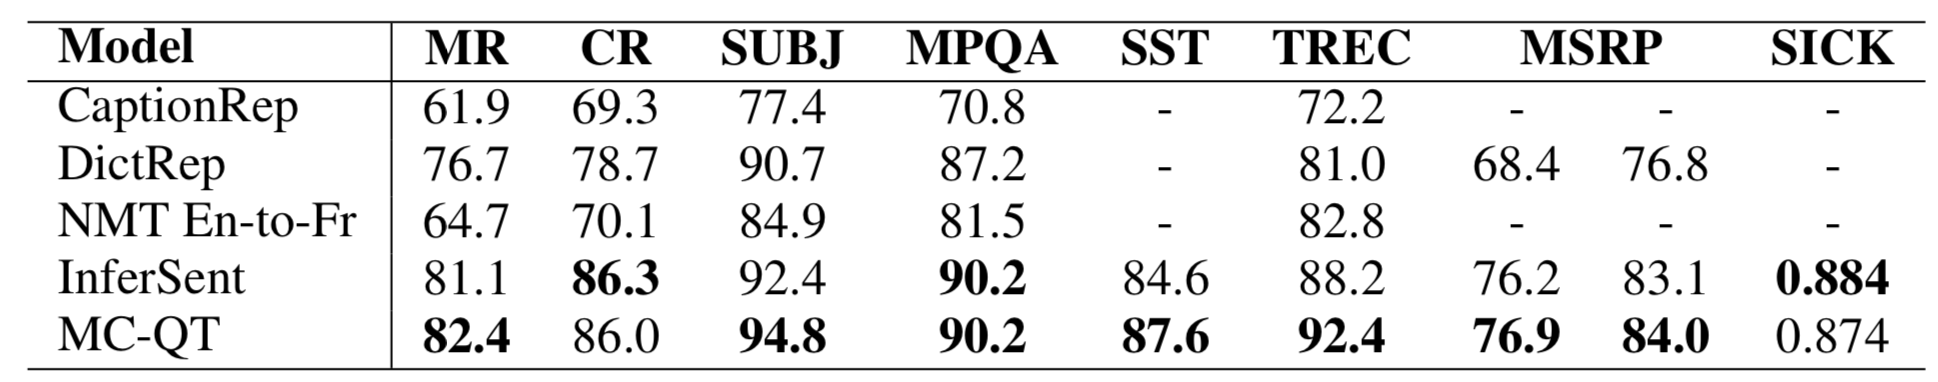
\includegraphics[width=1\linewidth]{files/quickthoughts-3.png}
  \caption{Caption XX}
  \label{fig:quickthoughts-res2}
\end{figure}

\begin{figure}[h!]
\centering
  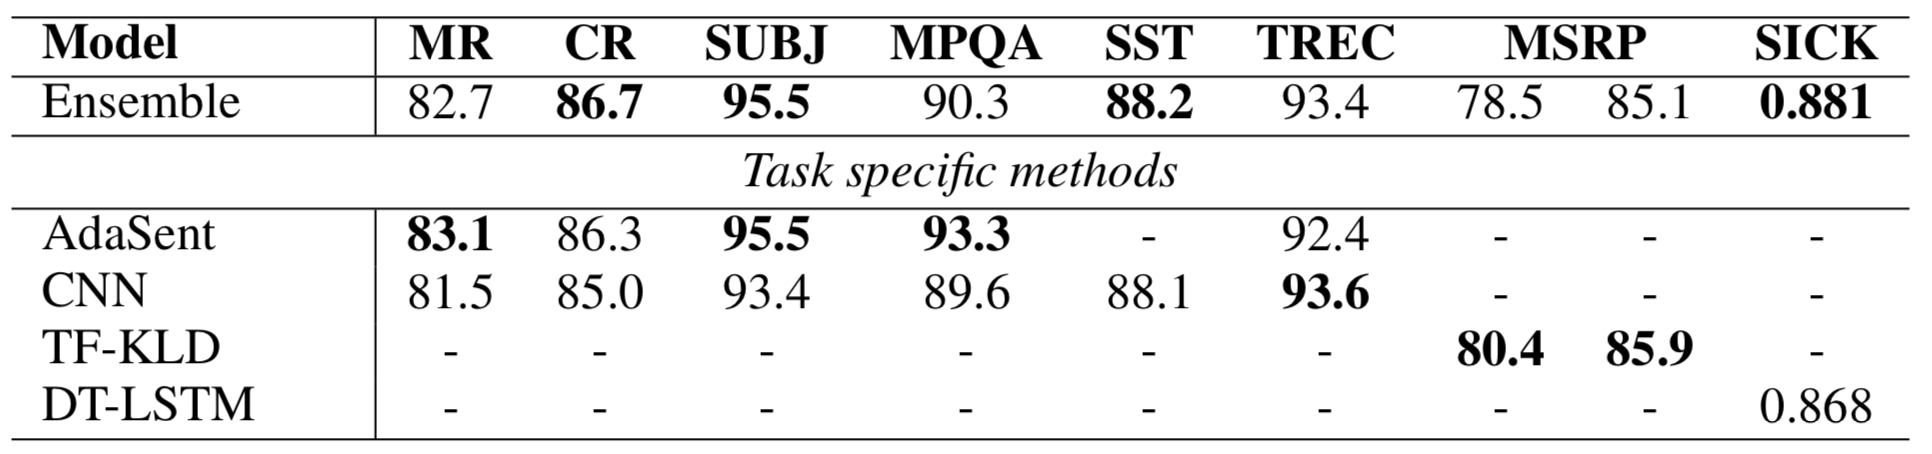
\includegraphics[width=1\linewidth]{files/quickthoughts-4.png}
  \caption{Caption XX}
  \label{fig:quickthoughts-res3}
\end{figure}

%\begin{figure}
%\centering
% 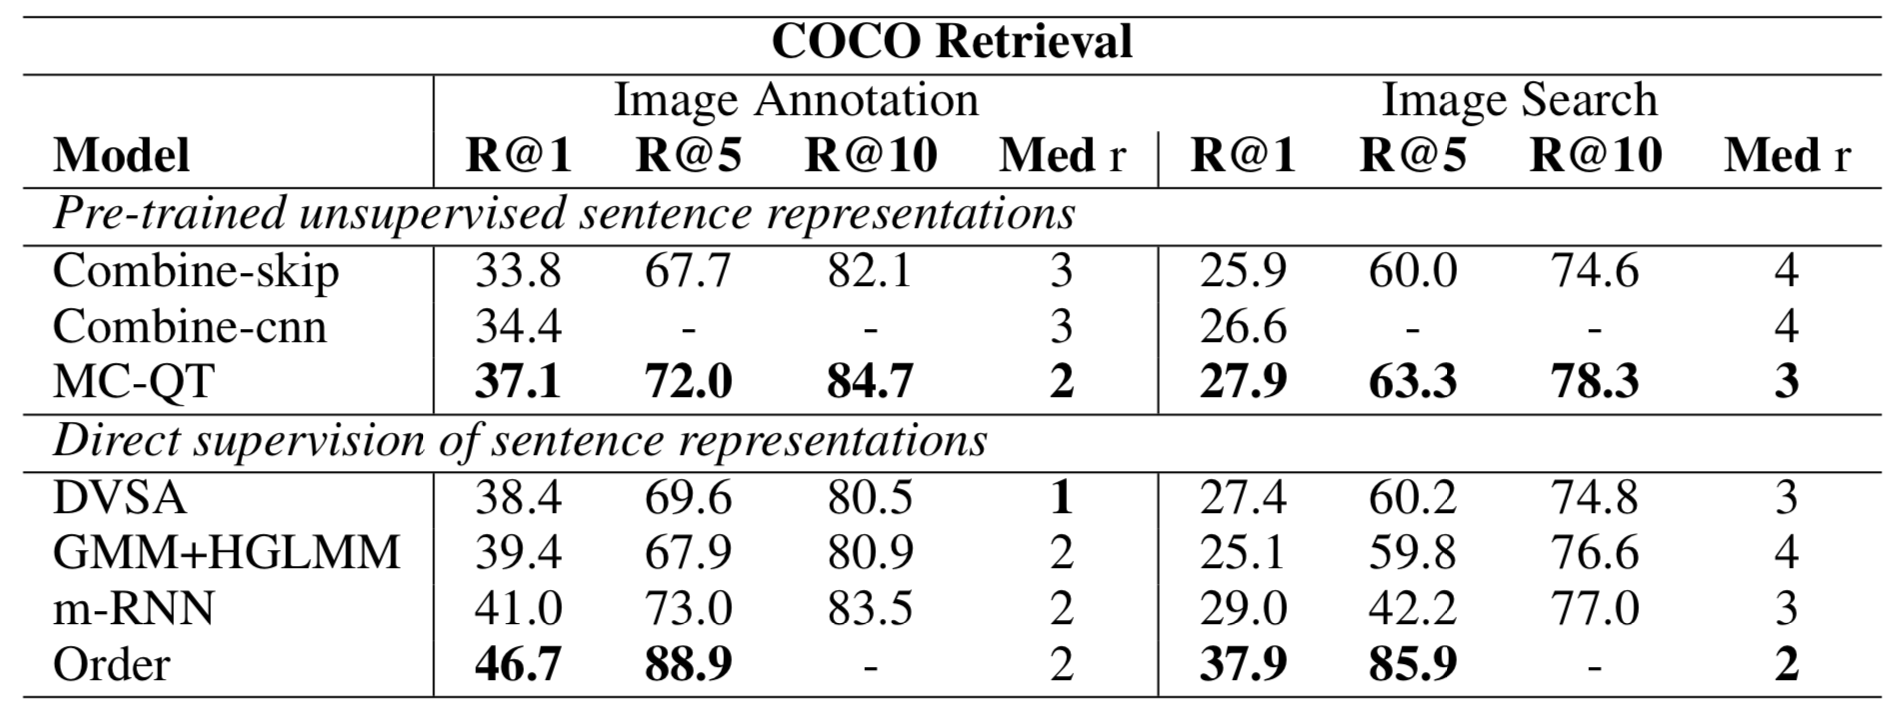
\includegraphics[width=.5\linewidth]{files/quickthoughts-5.png}
%  \caption{Cap.}
%  \label{fig:vae}
%\end{figure}

%\begin{figure}
%\centering
%  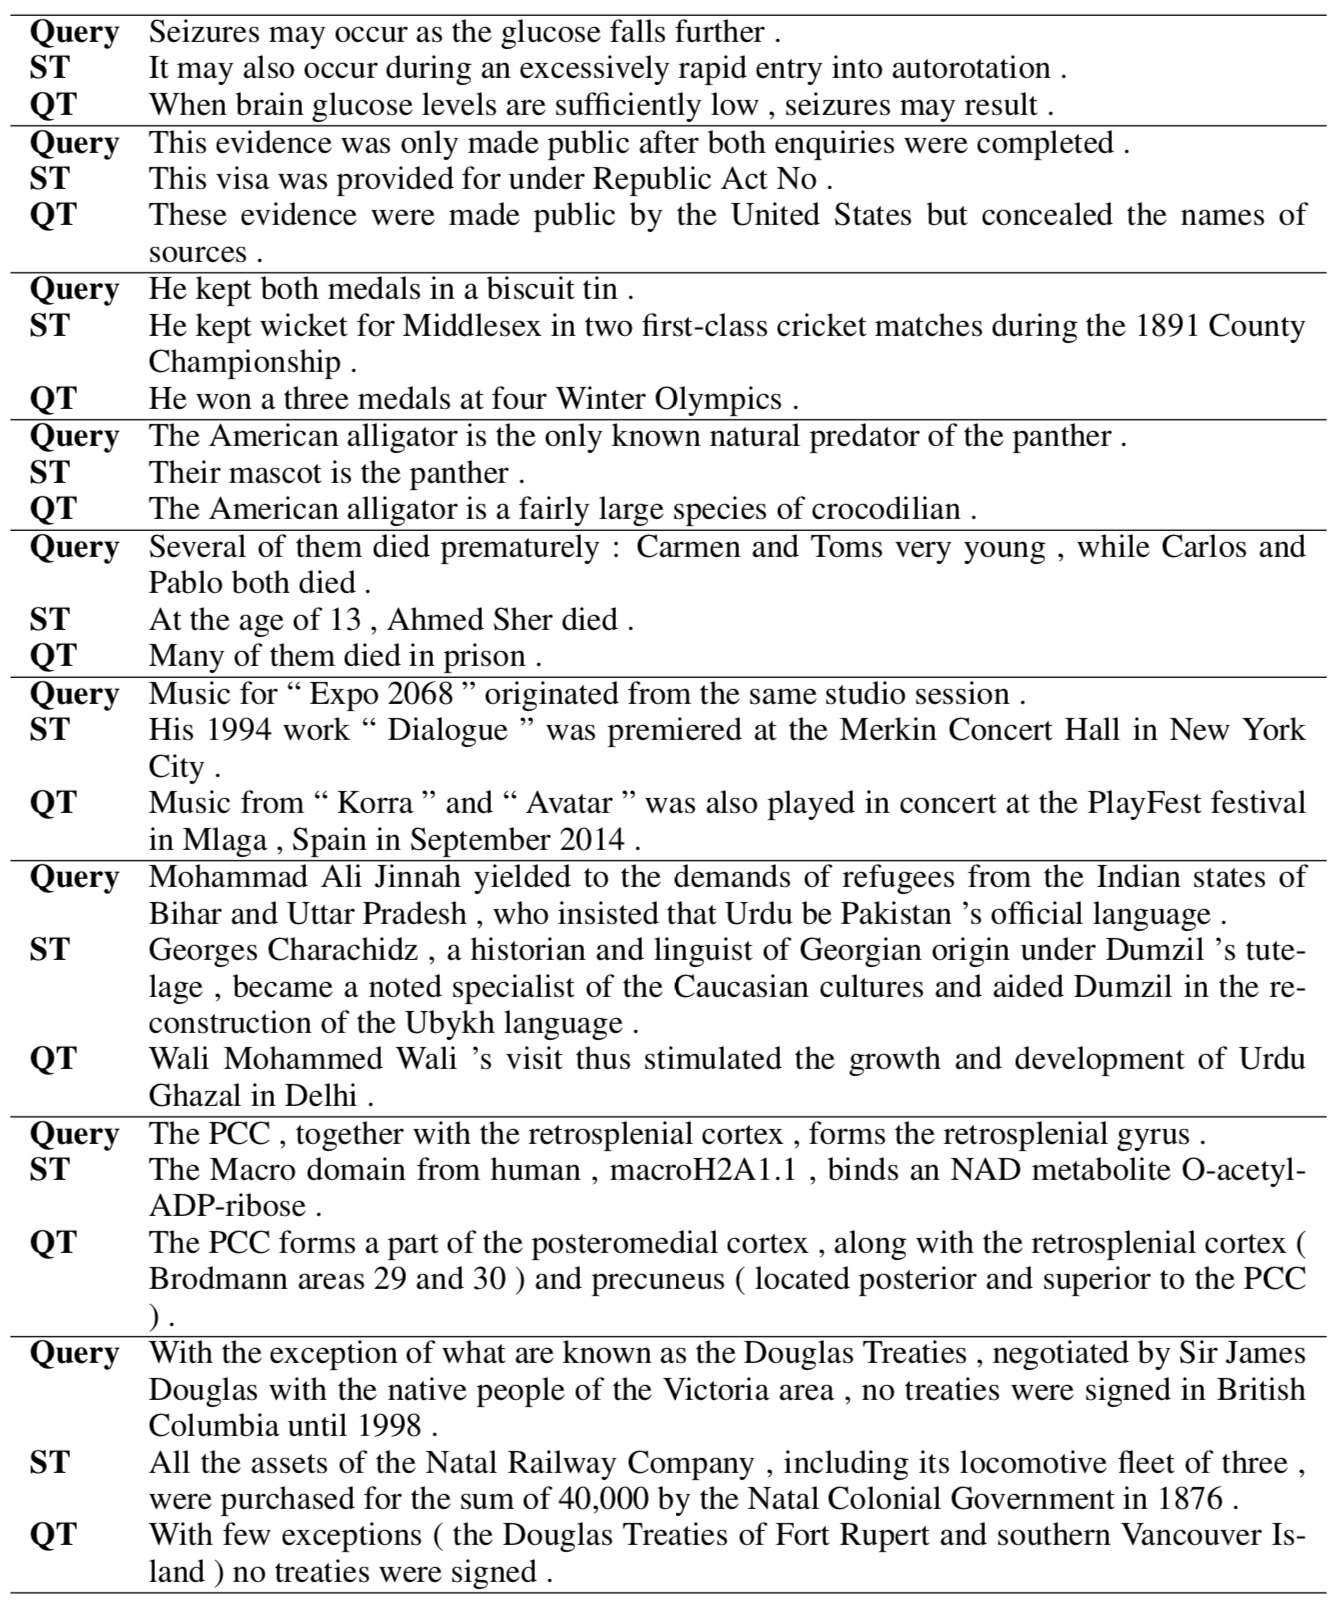
\includegraphics[width=.5\linewidth]{files/quickthoughts-6.png}
%  \caption{Cap.}
%  \label{fig:vae}
%\end{figure}

\subsection{Summary of Universal Sentence Encoder}
% TODO same as previous subsection

Due to the scarcity of training data, many NLP tasks rely on transfer learning by using pre-trained word or sentence embeddings. The universal sentence encoder (USE) \cite{use} are sentence embeddings designed for transfer learning with a model structure that targets weaknesses in applying pre-trained embeddings to new tasks. USE can be implemented with a transformer architecture or with a deep averaging network. These variants are designed to allow trade-offs between computational efficiency and accuracy. 

The transformer-based architecture has high accuracy but greater computational requirements. Self-attention \cite{attention} is used to create sentence embeddings that account for word order and importance. The model uses multi-task learning to foster generalizability by updating a single encoder based on performance on a skip-thought-like task using the transformer in place of the LSTM, a conversational input-response task, and supervised classification. The deep averaging network (DAN) approach generates a sentence encoding using the architecture proposed by \cite{dan}, sacrificing accuracy for reduced compute time.

USE is trained on a variety of web data, including Wikipedia, news, question-answer sites like Quara, and forums. This training set is supplemented with supervised data from the Stanford Natural Language Inference corpus. Transfer tasks for multi-task learning are tested with word-level transfer with pre-trained word2vec embeddings and with randomly initialized word embeddings that are learned for each task. Similarity for classification transfer tasks is calculated with angular distance rather than cosine similarity. Hyperparameters are tuned with cross-validation and Vizier. 

The transformer architecture tends to outperform the DAN encoder, espsecially for tasks with limited training data sets (Figure \ref{fig:use-2}) and models with pre-trained word embeddings tend to outperform those that learn word embeddings for tasks with small training data sets. While the transformer architecture performs remarkably better on small training sets than does DAN, the transformer only increases accuracy by one or two relative percentage points when sufficient training data is available (Figure \ref{fig:use-1}.) 

The compute time of the transformer is quadratically related to the sentence length and training size, while the compute time for the DAN architecture has a linear relationship. There is a similar relationship for memory usage. DAN is much less computationally intensive than the transformer architecture, and the authors suggest choosing between the approaches by considering the tradeoffs between memory, compute time, and accuracy. Ultimately, USE provides sentence embeddings that perform well when transferred to a variety of NLP tasks and allow the end-user to choose between accuracy and compute time.

\newpage


%\begin{figure}
%\centering
%  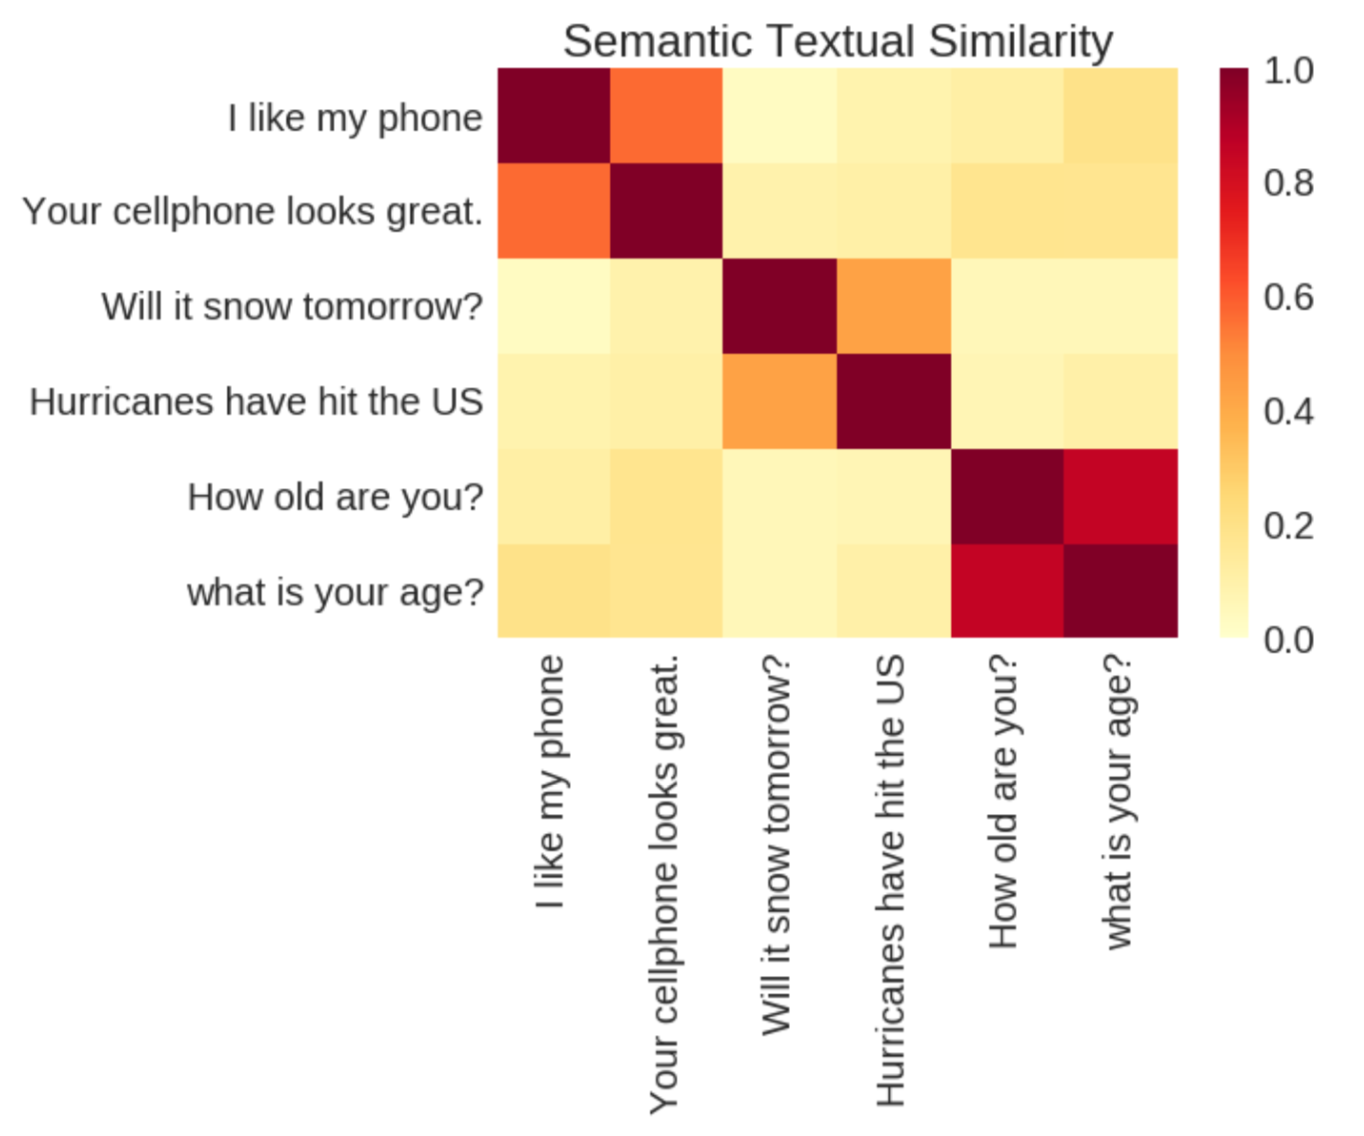
\includegraphics[width=1\linewidth]{files/use-1.png}
%  \caption{Cap.}
%  \label{fig:vae}
%\end{figure}

\begin{figure}[h!]
\centering
  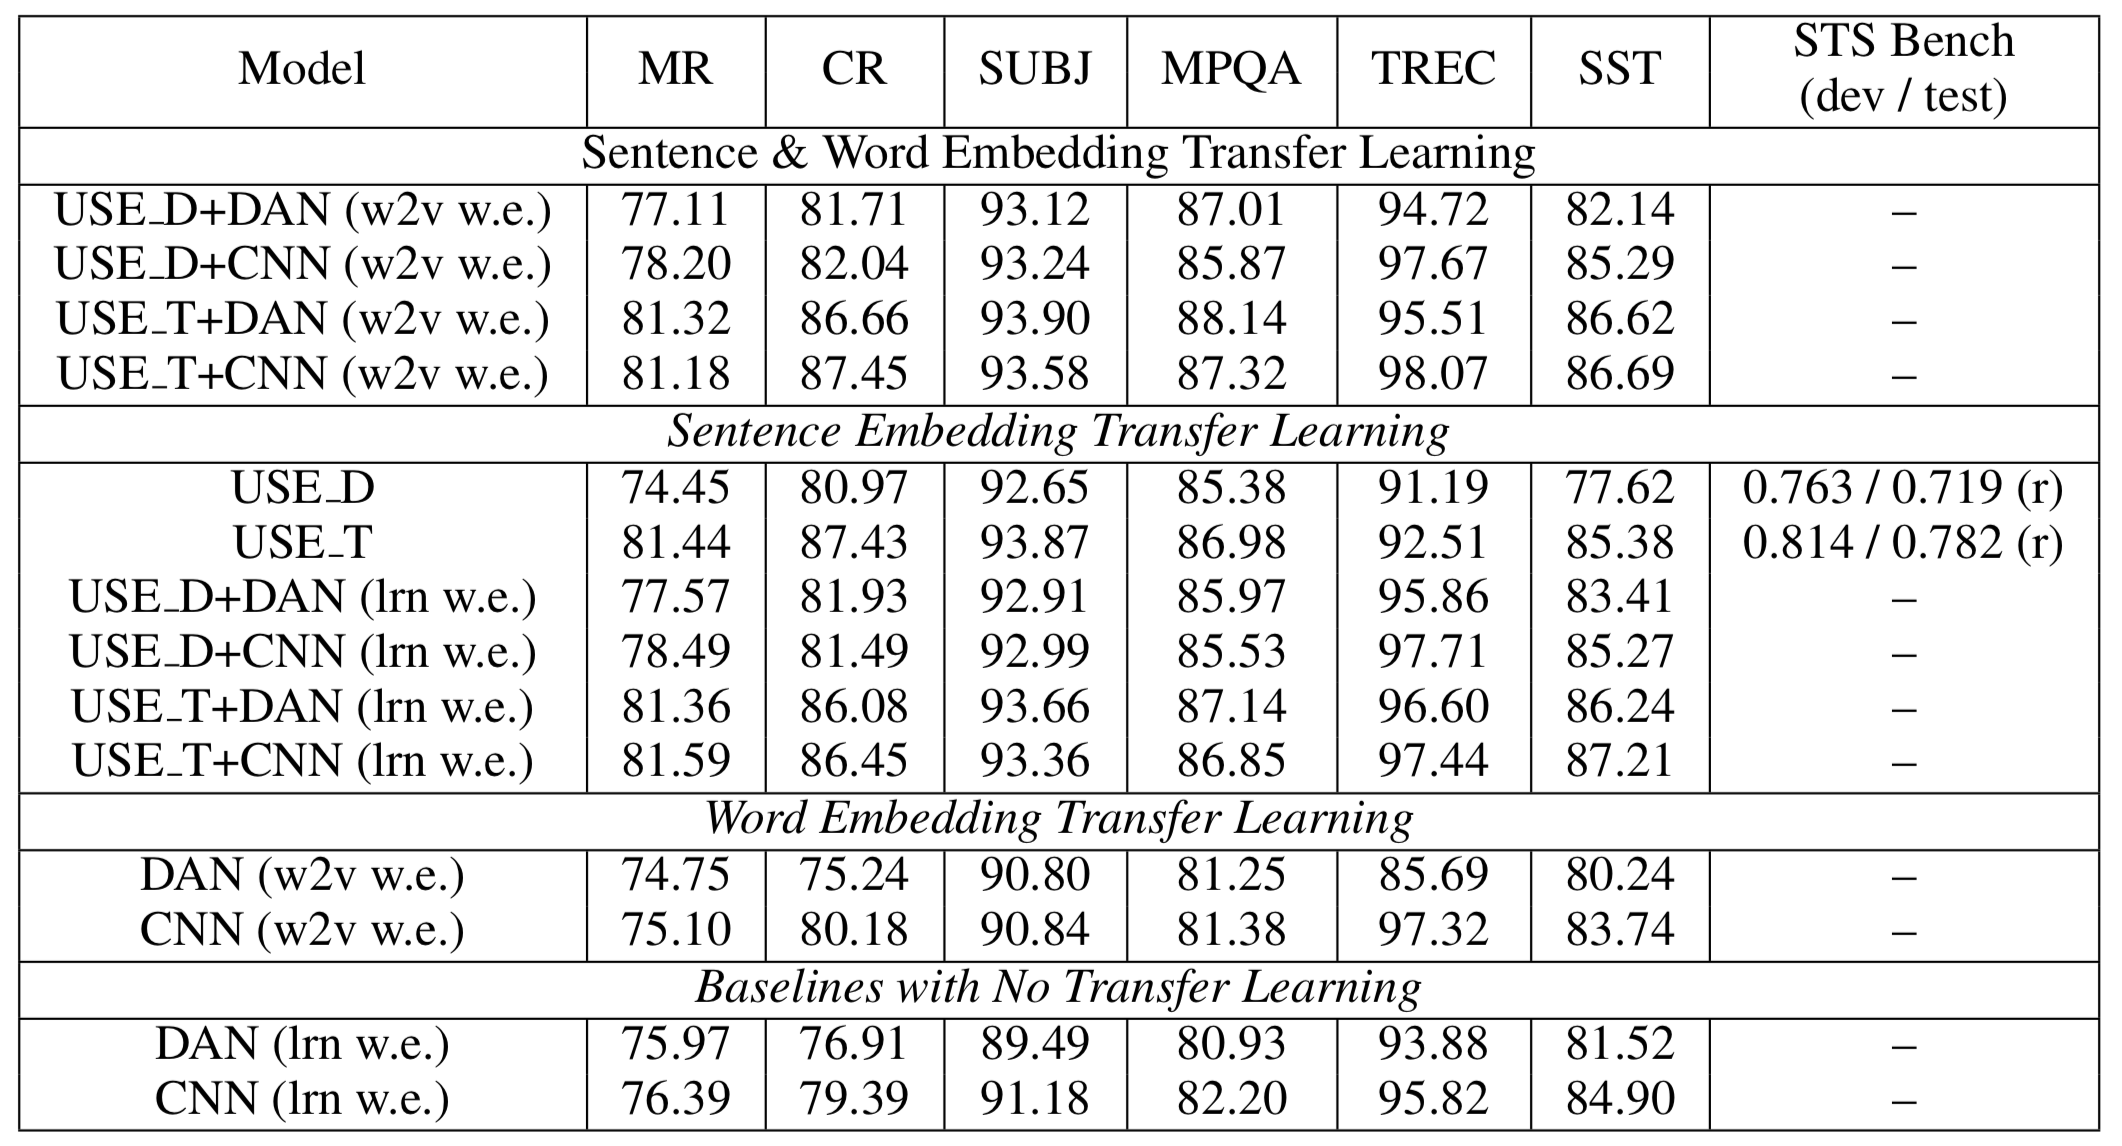
\includegraphics[width=1\linewidth]{files/use-2.png}
  \caption{Caption 1.}
  \label{fig:use-1}
\end{figure}

\begin{figure}[h!]
\centering
  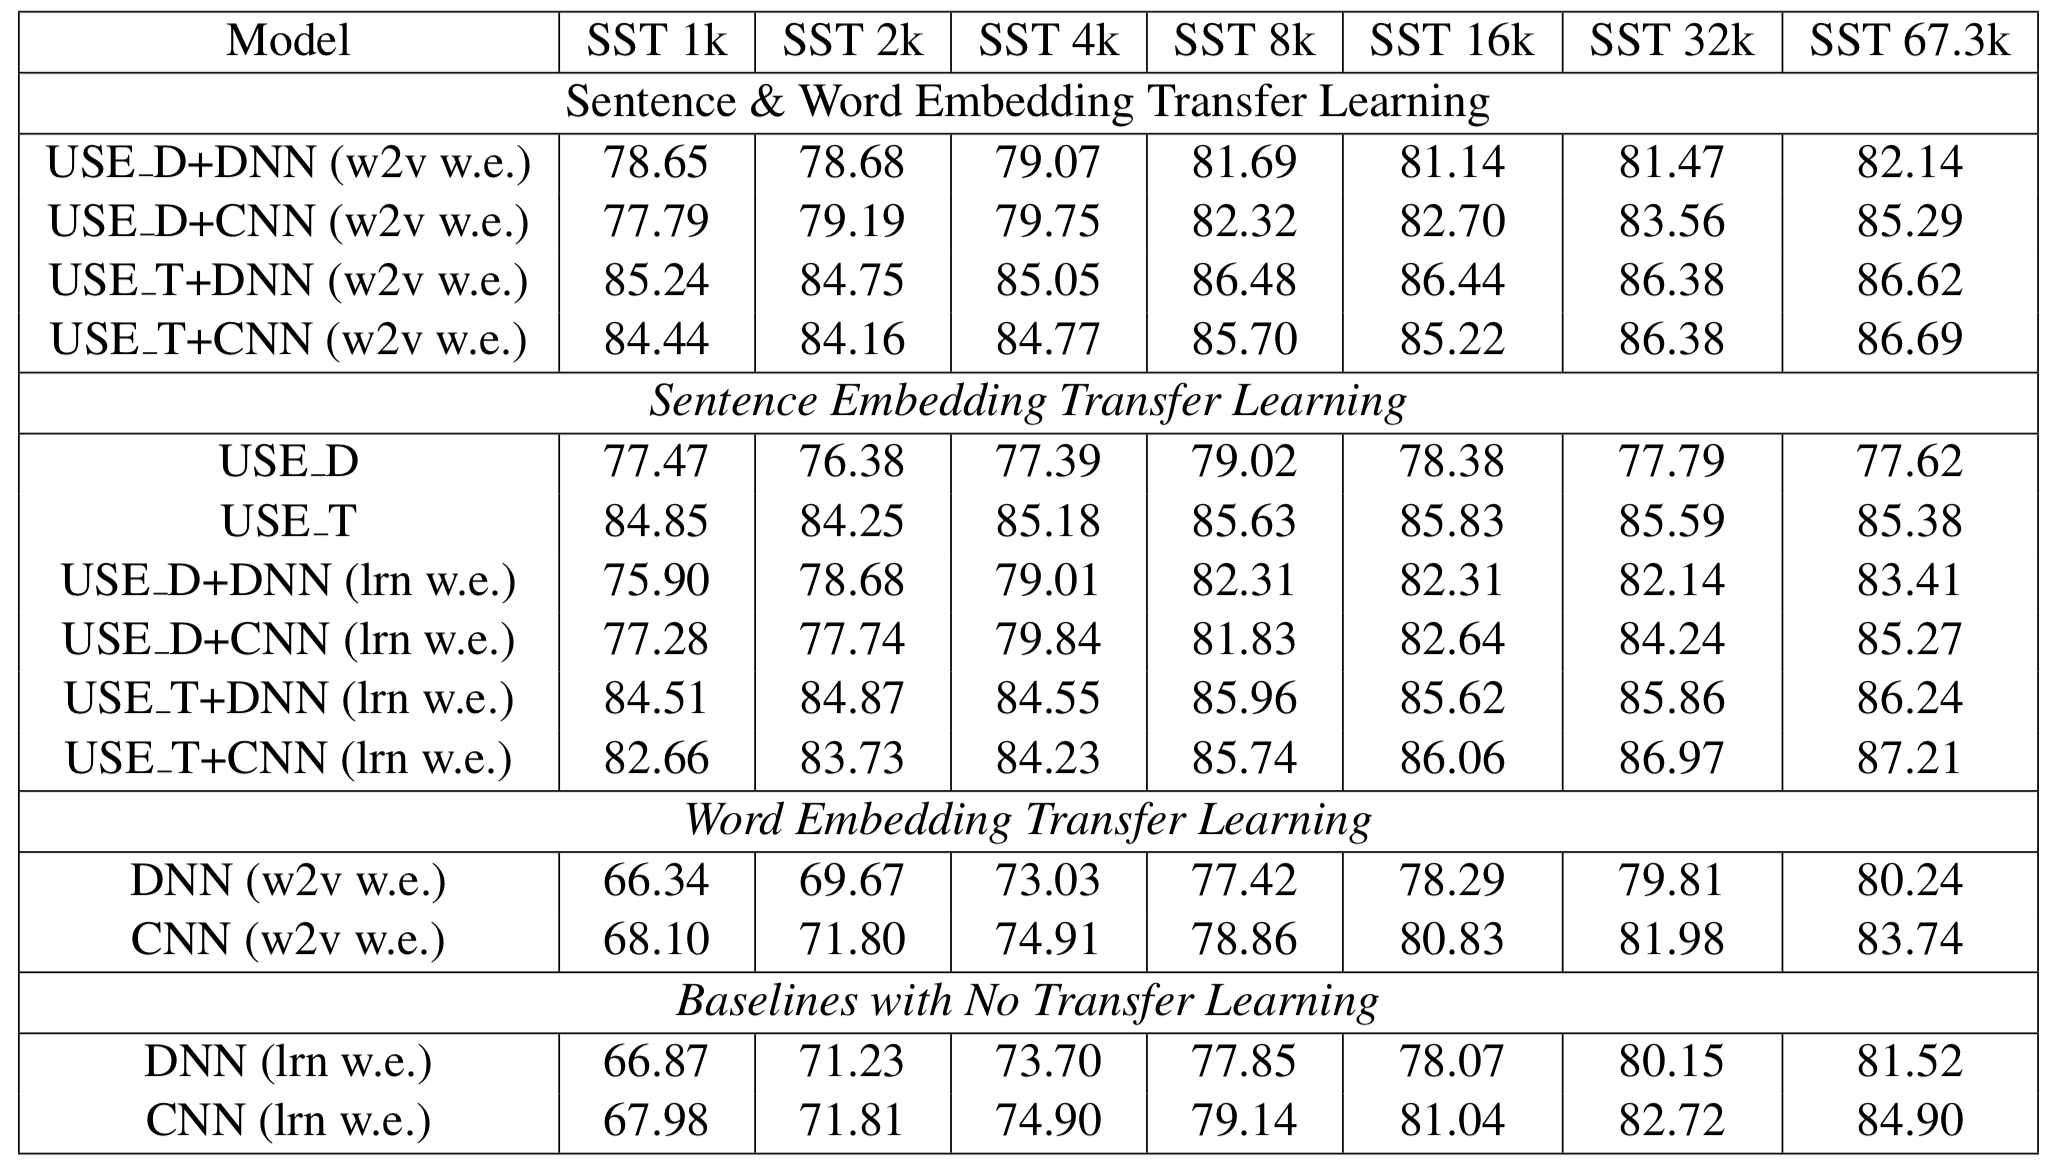
\includegraphics[width=1\linewidth]{files/use-3.png}
  \caption{Caption 2.}
  \label{fig:use-2}
\end{figure}

\newpage

\section{\label{sec:level5} Comparison of Papers}
% TODO Give a short overview/comparison of the methods discussed in the papers

\section{\label{sec:level6} Summary}
% Conclude the presentation/make any final brief statements. This is not a summary like the introduction. 
